% Build adapter for the unchanged historical source.
% It supplies the Unicode hyphen mapping, uses the deduplicated bibliography,
% and fits the one oversized portrait figure on its page. No prose is changed.
\RequirePackage[utf8]{inputenc}
\DeclareUnicodeCharacter{2010}{-}
\RequirePackage{xurl}
\AtBeginDocument{%
  \setlength{\emergencystretch}{3em}%
  \let\BaselineBibliography\bibliography
  \renewcommand{\bibliography}[1]{\BaselineBibliography{references_full_revision}}%
  \let\BaselineIncludeGraphics\includegraphics
  \renewcommand{\includegraphics}[2][]{%
    \ifnum\pdfstrcmp{#2}{quasi_potential_slices_sparse.png}=0
      \BaselineIncludeGraphics[width=0.94\textwidth]{#2}%
    \else
      \BaselineIncludeGraphics[#1]{#2}%
    \fi}%
}
\documentclass[11pt]{article}
\usepackage{amsthm}  
\usepackage{graphicx}
\usepackage[colorlinks,linkcolor=red]{hyperref} 
\usepackage{bigstrut,multirow,rotating} 
\usepackage{booktabs}            
\usepackage{enumerate}
\usepackage{amsmath}
\usepackage{bbm}
\usepackage{amsfonts,amssymb}
\usepackage{appendix, subcaption}
\usepackage[numbers,sort&compress]{natbib}
\usepackage[a4paper, margin=3cm]{geometry}
\usepackage{authblk} % <-- Add this for multiple authors/affiliations
\usepackage[mathlines]{lineno}
\linenumbers
% --- Theorem styles -------------------------------------------------
\theoremstyle{plain}      % default: bold header + italic body
\newtheorem{theorem}{Theorem}[section]     % theorem 3.2, 3.3, … within section 3
\newtheorem{lemma}[theorem]{Lemma}         % share counter with theorems
\newtheorem{proposition}[theorem]{Proposition}
\newtheorem{corollary}[theorem]{Corollary}

\theoremstyle{definition} % bold header + upright body
\newtheorem{definition}[theorem]{Definition}
\newtheorem{remark}[theorem]{Remark}

% optional: custom qed symbol for proofs that end with equations
\renewcommand{\qedsymbol}{$\square$}

\title{Kernel Methods for the Computation of Quasi-Potentials in Stochastic Dynamical Systems}

\author[1]{Jonghyeon Lee\thanks{jlee9@caltech.edu}}
\author[1,5]{Boumediene Hamzi\thanks{boumediene.hamzi@gmail.com. Parts of this work were carried out while BH was a resident scholar at the Isaac Newton Institute for Mathematical Sciences, Cambridge, UK.}}
\author[2]{Yang Li \thanks{Corresponding author: liyangbx5433@163.com}}
\author[1]{Houman Owhadi\thanks{owhadi@caltech.edu}}
\author[3]{Umesh Vaidya\thanks{uvaidya@clemson.edu}}
\author[4]{Naiming Xie\thanks{xienaiming@nuaa.edu.cn}}

\affil[1]{Department of Computing and Mathematical Sciences, Caltech, CA, USA}
\affil[2]{School of Automation, Nanjing University of Science and Technology, Nanjing 210094, China}
\affil[3]{Department of Mechanical Engineering, Clemson University Clemson, SC, USA}
\affil[4]{Nanjing University of Aeronautics and Astronautics, Nanjing 210094, China}
\affil[5]{The Alan Turing Institute, London, UK}


\date{}

\begin{document}

  \maketitle

 
\begin{abstract}
We present a data-driven, kernel-based framework for reconstructing the quasi-potential of stochastic differential equations (SDEs) in the weak-noise regime.  
The method approximates a family of Koopman eigenfunctions in a reproducing-kernel Hilbert space and combines them into a closed-form surrogate whose gradient automatically satisfies a quadratic Hamilton–Jacobi ansatz.  
A composite loss simultaneously (i) minimises the Hamilton–Jacobi residual on a collocation grid, (ii) matches the Hessian of the surrogate to the solution of the Riccati equation at the equilibrium, and (iii) promotes sparsity through an \(\ell_{1}\) penalty on the kernel-mixture weights.  

Numerical experiments show that the analytic surrogate is inexpensive to evaluate, paving the way for efficient rare-event analysis and optimal-control applications in higher-dimensional, non-gradient stochastic systems.
\end{abstract}

\section{Introduction}
\label{intro}
Noise-induced transitions and rare escape phenomena are ubiquitous in physical, chemical, biological, and engineering systems \cite{horsthemke1984noise, zhu2003first}. The Freidlin-Wentzell large deviation theory serves as a fundamental framework for analyzing rare events driven by weak noise \cite{Freidlin2012, 10.1214/07-AOP362, dean2009splitting, huisinga2003extracting, lu2017gaussian}. Central to this theory is the concept of the action functional, which quantifies the likelihood of trajectories deviating from deterministic paths. The quasi-potential, defined as the infimum of the action functional, lies at the heart of large deviation theory. It characterizes the probability of a stochastic system fluctuating into a neighborhood of a specific state and governs key quantities such as mean first exit times and stationary distributions.

Despite its importance, computing the quasi-potential remains challenging. Traditional approaches can be categorized into three classes. Action Plot Methods \cite{beri2005solution}: These methods parameterize trajectories by integrating along unstable manifolds in the extended Hamiltonian phase space, starting from a small circle near a fixed point until exiting the basin of attraction. While effective for obtaining quasi-potential values along parameterized paths, they fail to establish a direct relationship between the quasi-potential and spatial coordinates. Geometric Minimum Action Method (GMAM) \cite{heymann2008geometric}: As a representative of string methods \cite{grafke2019numerical, zhou2008adaptive, cameron2011string, weinan2004minimum}, GMAM iteratively identifies the most probable path between a fixed point and a target state. However, it computes the quasi-potential only at discrete endpoints, lacking global structure. Ordered Upwind Method (OUM) \cite{cameron2012finding, dahiya2018ordered}: By discretizing the phase space and propagating quasi-potential values outward from fixed points, OUM achieves global quasi-potential reconstruction. Yet, its computational efficiency remains limited, especially in high-dimensional systems.

Recent advances in computational power and artificial intelligence have spurred the application of machine learning to stochastic dynamics. Techniques such as sparse regression \cite{Boninsegna2018, YangLi2020a}, Koopman operators \cite{EDMD, SKO3}, and neural networks \cite{XiaoliChen} have been leveraged for data-driven modeling of stochastic systems. In addition, some machine learning methods are also proposed to solve the problem of noise-induced transitions such as computing the most probable paths \cite{li2021machine, wei2022optimal} and the mean first exit times \cite{li2024deep}. Notably, Lin et al. \cite{lin2022data} proposed neural network-based frameworks to compute quasi-potentials for stochastic dynamical systems with additive Gaussian noise, while Li et al. \cite{li2022machine} developed physics-informed neural networks (PINNs) to compute quasi-potentials by solving Hamilton-Jacobi equations.

Among machine learning paradigms, kernel methods stand out due to their strong nonlinear representation capabilities and computational efficiency. Notably, reproducing kernel Hilbert spaces (RKHS) \cite{CuckerandSmale} have established solid mathematical foundations for the analysis of  dynamical systems \cite{BH4, yk1, bhcm11,bhcm1, lyap_bh, bh_sparse_kfs, BHPhysicaD, hamzi2019kernel, bh2020b,SKO3,ALEXANDER2020132520,bh12,bh17,hb17,mmd_kernels_bh, hamzipaillet,jalalian_deds_2023,lee2024note, hamzi2025kernel_lions, bittracher2021dimensionality} and surrogate modeling (cf.\ \cite{santinhaasdonk19} for a survey) as well as analyzing neural networks \cite{smirnov2022mean}. \textcolor{red}{The idea of combining multiple kernels by learning a weighted mixture is known as \emph{multiple kernel learning} (MKL) \cite{lanckriet2004learning, bach2004multiple} and has been studied extensively in the machine learning literature. Our approach is related to MKL in that we learn a sparse convex combination of base kernels, but it differs in that the objective couples kernel selection with PDE residual minimization and curvature matching, rather than regression or classification loss.}

In this work, we present a kernel-based algorithm for quasi-potential computation. The structure of this paper is as follows: \textcolor{red}{Section~\ref{qpsec} introduces the definition and properties of the quasi-potential. Section~\ref{methsec} details the proposed kernel-driven methodology. Numerical examples in Section~\ref{examples} validate the algorithm's accuracy and efficiency, followed by concluding remarks.}



%\section{Quasi-potential}

%Stochastic dynamical systems of the form
%\begin{equation}
%  dx_t = b(x_t) dt + \sqrt{\varepsilon}\,\sigma(x_t) dB_t
%\end{equation}
%model various phenomena where deterministic dynamics are influenced by noise. Here, \(\varepsilon\) is small, indicating weak noise, and \(B_t\) is a standard Brownian motion. The system tends to dwell near stable fixed points of the deterministic dynamics, occasionally making transitions due to noise.

%A key tool to study such transitions is the \emph{quasi-potential} \(V(x)\), which quantifies the most probable path of escape and transition probabilities. When the noise is weak, the stationary distribution takes the WKB form:
%\begin{equation}
%  p_s(x) \sim C(x)\,\exp(-\varepsilon^{-1} V(x))
%\end{equation}
%where \(V(x)\) solves a Hamilton-Jacobi equation (HJE):
%\begin{equation}
%  H(x, \nabla V) = b(x)^T \nabla V + \tfrac{1}{2} \nabla V^T a(x) \nabla V = 0
%\end{equation}
%with \(a(x) = \sigma(x) \sigma(x)^T\).


 


 

\setcounter{equation}{0}
\section{Quasi-Potential and the Wentzel–Kramers–Brillouin Approximation in Stochastic Dynamical Systems} \label{qpsec}

In this section, we examine dynamical systems governed by state variables \( x_t \in \mathbb{R}^n \), evolving under the influence of Gaussian white noise with low intensity. The dynamics are described by the stochastic differential equation:
\begin{equation}
\label{sde}
dx_t = b(x_t)\,dt + \sqrt{\varepsilon}\,\sigma(x_t)\,dB_t,
\end{equation}
\iffalse
where \( B_t \in \mathbb{R}^n \) denotes an \( n \)-dimensional standard Brownian motion, and \( \varepsilon \) is a small positive parameter quantifying the noise strength. \textcolor{red}{The function \( b(x) \in \mathbb{R}^n \) represents the deterministic drift term which has continuously differentiable derivatives,} while the diffusion coefficient is given by the matrix \( a(x) = \sigma(x)\sigma(x)^T \).

% REPLACE existing text after Equation (2) with:
\fi
where $B_t \in \mathbb{R}^n$ denotes an $n$-dimensional standard Brownian motion, and $\varepsilon$ is a small positive parameter quantifying the noise strength. The function $b(x) \in \mathbb{R}^n$ represents the deterministic drift term, which we assume has continuously differentiable derivatives. The diffusion coefficient is given by the matrix $a(x) = \sigma(x)\sigma(x)^\top$, where we assume $a(x)$ is uniformly positive definite on $\Omega$ (ensuring non-degeneracy of the noise).

We suppose $\bar{x}$ is an \textbf{asymptotically stable and hyperbolic} fixed point of the associated deterministic system, that is, $b(\bar{x}) = 0$ and all eigenvalues of its linearization matrix $J = \nabla b(\bar{x})$ have \textbf{strictly negative real parts}, i.e., $\text{Re}(\lambda_i) < 0$ for all $i = 1,\ldots,n$. This ensures asymptotic stability in the sense that trajectories starting near $\bar{x}$ converge to $\bar{x}$ exponentially in time. Under stochastic perturbations, the process $x_t$ explores the state space and converges to a stationary probability distribution $p_s(x)$. In the regime of weak noise ($\varepsilon \ll 1$), this stationary distribution admits a Wentzel--Kramers--Brillouin (WKB)-type asymptotic approximation (see \cite{chen2017singularities,li2022machine,smelyanskiy1997topological}):
\begin{equation}
\label{WKB}
p_s(x) \sim C(x)\, \exp\left\{-\varepsilon^{-1} V(x)\right\},
\end{equation}
where \( C(x) \) is a slowly varying prefactor and \( V(x) \) is the quasi-potential function, characterizing the exponential decay rate of the probability density. This form is termed a \emph{WKB-type approximation} named after the WKB method in quantum mechanics, where solutions in the semiclassical limit \( \hbar \to 0 \) take the form \( \psi(x) \sim A(x)\exp\{i S(x)/\hbar\} \). In both contexts, the exponential term dominates and captures the leading-order behavior, while the prefactor varies more slowly. In stochastic systems, the small parameter \( \varepsilon \) appears in the exponent, leading to sharp concentration of the probability distribution around stable points as \( \varepsilon \to 0 \). The quasi-potential \( V(x) \) acts as an effective potential or energy landscape, quantifying the cost of rare fluctuations. The symbol ``\( \sim \)'' denotes logarithmic equivalence, meaning that
\[
\lim_{\varepsilon \to 0} \frac{\log p_s(x)}{-\varepsilon^{-1} V(x)} = 1,
\]
which highlights that \( V(x) \) governs the leading-order behavior in the small noise limit.

The concept of the quasi-potential originates from large deviation theory \cite{Freidlin2012}. It is defined via a variational principle involving the Freidlin–Wentzell action functional \( S_T[\phi] \), formulated over continuous trajectories \( \phi(t) \) that connect a stable fixed point \( \bar{x} \) to a target point \( x \). Specifically, the quasi-potential is given by the nested infimum:
\begin{equation}
\label{quasip}
V(x) \equiv \inf_{T > 0} \inf_{\phi \in C([0, T])} \left\{ S_T[\phi] \,:\, \phi(0) = \bar{x},\; \phi(T) = x \right\},
\end{equation}
where \( C([0,T]) \) denotes the space of continuous functions on the interval \([0, T]\). The action functional \( S_T[\phi] \), fundamental in the large deviation framework, is given by
\begin{equation}
\label{actionf}
S_T[\phi] = \int_0^T L(\phi(t), \dot{\phi}(t))\,dt,
\end{equation}
with the Lagrangian \( L(\phi, \dot{\phi}) \) for the stochastic differential equation \eqref{sde} defined as follows
\begin{equation}
\label{Lagran}
L(\phi, \dot{\phi}) = \frac{1}{2} \left[ \dot{\phi} - b(\phi) \right]^{\!\!T} a^{-1}(\phi) \left[ \dot{\phi} - b(\phi) \right].
\end{equation}

This action functional quantifies the cost of deviations from the deterministic path and plays a central role in describing the asymptotic probability of rare events. In particular, for a fixed trajectory \( \phi(t) \), the probability that the stochastic process \( x_t \) remains within a small tube around \( \phi(t) \) over the time interval \([0, T]\) satisfies the large deviation estimate:
\begin{equation}
\label{LDP}
\mathbb{P}_{x_0} \left\{ \sup_{t \in [0, T]} \left| x_t - \phi(t) \right| < \delta \right\} \sim \exp\left\{ -\varepsilon^{-1} S_T[\phi] \right\},
\end{equation}
for small \( \delta > 0 \), illustrating that the action functional governs the exponential rate of decay of such pathwise probabilities.

Note that the stationary probability distribution satisfies the time-independent Fokker–Planck equation 
\[ \mathcal{L}p_s(x) = - \sum_{i=1}^n \frac{\partial}{\partial x_i} b_i(x)p_{s}(x) + \sum_{i,j=1}^n \frac{\partial^2}{\partial x_i \partial x_j} a_{ij}(x)p_{s}(x) = 0, \]
where \( \mathcal{L} \) is the Fokker–Planck operator. Substituting the WKB ansatz \eqref{WKB} into this equation and collecting the leading-order terms in \( \varepsilon \) yields the Hamilton–Jacobi equation:
\begin{equation}
\label{HJE}
H(x, p) \equiv b^{T}p + \frac{1}{2} p^{T}ap = 0, \quad p \equiv \nabla V (x),
\end{equation}
which is a first-order nonlinear partial differential equation for the quasi-potential \( V \). It is observed that this Hamiltonian is the Legendre transform of the Lagrangian \eqref{Lagran}. According to the definition \eqref{quasip}, the quasi-potential at the fixed point satisfies \( V(\bar{x}) = 0 \). Since the quasi-potential function attains minimal value at the stable fixed point, the gradient of the quasi-potential is also zero at the stable point, i.e., $\nabla V(\bar{x}) =0$.

If \( b(x) = -\nabla U(x) \) (i.e., a gradient system) and \( a(x) = I \) (i.e., additive noise), then the quasi-potential function equals twice the potential: \( V(x) = 2U(x) \). In this special case, the quasi-potential admits an analytical expression.

Assume that the second-order approximation of the quasi-potential function at the fixed point \( \bar{x} \) is given by
\[
\begin{aligned}
V(x) & \approx V(\bar{x}) + \nabla V(\bar{x}) (x - \bar{x}) + \frac{1}{2} (x - \bar{x})^T \nabla^2 V(\bar{x}) (x - \bar{x}) \\
& = \frac{1}{2} (x - \bar{x})^T Z (x - \bar{x}),
\end{aligned}
\]
where \( Z = \nabla^2 V(\bar{x}) \). Consequently, its gradient is approximated as
\[
\nabla V(x) \approx Z (x - \bar{x}).
\]
Substituting the gradient approximation into the Hamilton–Jacobi equation (\ref{HJE}) yields
\begin{equation}\label{HJE2}
b(x)^T Z (x - \bar{x}) + \frac{1}{2} (x - \bar{x})^T Z^T a(x) Z (x - \bar{x}) \approx 0.
\end{equation}
Near the fixed point, we also approximate the drift $b(x)$ and the diffusion $a(x)$ as
\[
b(x) \approx F(x-\bar{x}), \ a(x) \approx A,
\]
where $F \equiv \nabla b(\bar{x}), A \equiv a(\bar{x})$. Substituting the linearized $b(x)$ and $a(x)$ into Eq. (\ref{HJE2}), we have
\begin{equation}\label{HJE3}
(x - \bar{x})^T (F^TZ + \frac{1}{2} Z^TAZ) (x - \bar{x}) \approx 0.
\end{equation}
Note that it is equivalent to the following equation.
\begin{equation}\label{HJE4}
(x - \bar{x})^T (F^TZ + ZF + Z^TAZ) (x - \bar{x}) \approx 0.
\end{equation}
\textcolor{red}{Since the matrix $F^TZ + ZF + Z^TAZ$ is a symmetric matrix, it must be diagonalizable. Due to the arbitrariness of $x - \bar{x}$, the eigenvalues of the matrix must all be 0. That is, each element of the matrix is 0.} Therefore, the Hessian matrix \( Z = \nabla^2 V(\bar{x}) \) satisfies the algebraic Riccati equation:
\begin{equation}\label{HJE5}
 F^TZ + ZF + Z^TAZ= 0
\end{equation}
or the equivalent form:
\begin{equation}
\label{Riccati}
FZ^{-1} + Z^{-1}F^T + A = 0.
\end{equation}

The principal challenge in computing the quasi-potential from the PDE \eqref{HJE} lies in avoiding trivial solutions. To address this, we employ kernel methods to solve the PDE \eqref{HJE}, and use equation \eqref{Riccati} to impose that the Hessian of \( V \) at the origin coincides with the matrix \( Z \) solving \eqref{Riccati}.

It is worth emphasizing that the quasi-potential plays a pivotal role not only in large deviation theory but also in stochastic dynamics, as it is linked to various physical quantities. For example, the expected time to exit the domain of attraction of a fixed point—known as the mean exit time—is exponentially determined by the minimum of the quasi-potential on the boundary of the domain. The exit location distribution and the invariant measure can also be approximated based on the quasi-potential. Furthermore, once the quasi-potential function is known, the most probable transition path connecting two steady states can be derived from the quasi-potential. Typically, the most probable path passes through a saddle point, with the latter half of the trajectory beyond the saddle point following its unstable manifold toward the destination steady state. The first half of the path is obtained by solving the equation \begin{equation}\label{mppcomp}
\dot{x} = b(x) + a(x) \nabla V(x).
\end{equation}
The boundary conditions are $x(-\infty)=\bar{x}$ and $x(\infty)=x_{sa}$, where $x_{sa}$ denotes the saddle point. In practice, Equation (\ref{mppcomp}) is obtained by substituting $p= \nabla V(x)$ into the state equation $\dot{x} = b(x) + a(x)p$ of the Hamiltonian system corresponding to the Hamilton-Jacobi Equation (\ref{HJE}). Therefore, the most probable path is the projection of a heteroclinic orbit in the four-dimensional Hamiltonian phase space onto the two-dimensional space. For further properties of the quasi-potential, see \cite{Freidlin2012}. \begin{remark}
When $\varepsilon = 0$ (i.e. when there is no noise), our work will reduce to constructing the Lyapunov function for the unforced system $\dot{x} = b(x)$ \cite{giesl2019approximation, lee2024note}
\end{remark}


\section{Method for Approximating the Quasi-Potential}\label{methsec}

To approximate the quasi-potential, we exploit the spectral structure of the Koopman operator. Specifically, we construct eigenfunctions \( \varphi_i(x) \) satisfying the linear advection-type partial differential equations:
\begin{equation}
\nabla \varphi_i(x) \cdot b(x) = \lambda_i \varphi_i(x), \quad \varphi_i(\bar{x}) = 0, \quad \nabla \varphi_i(\bar{x}) = e_i,
\end{equation}
where \( \lambda_i \) are eigenvalues of the linearization \( J = \nabla b(\bar{x}) \) at the fixed point \( \bar{x} \), and \( e_i \) are the standard basis vectors. These eigenfunctions correspond to the Koopman eigenfunctions associated with the equilibrium dynamics and encode local geometric and dynamical information such as the structure of stable and unstable manifolds.

Let \( \Phi(x) = (\varphi_1(x) \cdots \varphi_n(x))^T \), and define the matrix \( W \) whose columns are the eigenvectors \( w_i \) of \( J \), satisfying \( J w_i = \lambda_i w_i \). We then define a quadratic approximation to the quasi-potential:
\begin{equation} \label{eq:vmid}
V_{\text{mid}}(x) = \tfrac{1}{2} \Phi(x)^T P_{\text{mid}} \Phi(x),
\end{equation}
with the symmetric matrix\footnote{Alternatively, one can set \( P_{\text{mid}} = \frac{1}{2}(P_u + P_\ell) \), where \( P_u \) and \( P_\ell \) solve Riccati-type equations: \( P \Lambda + \Lambda^\top P + PRP = 0 \), for different choices of \( R \).}:
\begin{equation}
P_{\text{mid}} = W\,\mathrm{diag}(-2\lambda_i)\,W^{-1}.
\end{equation}

To represent \( \varphi_i(x) \), we employ a data-driven kernel-based ansatz:
\begin{equation}\label{phiix}
\varphi_i(x) = \sum_{p=1}^N \alpha_p^{(i)}\,k_\beta(x, x_p) + (x - \bar{x}) \cdot w_i,
\end{equation}
where the point set \( \{ x_p \}_{p=1}^N \) denotes the collocation set which is used for training, and \( k_\beta(x, t) \) is a convex combination of base kernels (e.g., polynomials and radial basis functions), parameterized by a non-negative weight vector \( \beta \). This kernel formulation ensures flexibility and regularization, and it circumvents the need to construct the Koopman operator explicitly.

The coefficients $\alpha_p$ are determined by minimizing the regularized empirical loss functional using the representer theorem.   
To determine the coefficients $\alpha^{(i)} = (\alpha^{(i)}_1,\dots,\alpha^{(i)}_N)$,
we enforce the Koopman eigenfunction equation at the collocation points.
Specifically, for each $i=1,\dots,n$, we impose the conditions
\[
\varphi_i(\bar x)=0, \qquad
\nabla\varphi_i(\bar x)=e_i,
\]
together with the PDE constraint
\[
\nabla\varphi_i(x_p)\cdot b(x_p)
= \lambda_i\,\varphi_i(x_p),
\qquad p=1,\dots,N.
\]
Substituting the RKHS ansatz (\ref{phiix}) into these conditions yields a linear
system for the coefficients $\alpha^{(i)}$, which we solve in a
regularized least--squares sense:
\begin{equation}
    \label{eqn:alpha_eqn}
\min_{\alpha^{(i)}} \;
\sum_{p=1}^N 
\left(
\nabla\varphi_i(x_p)\cdot b(x_p)
- \lambda_i\,\varphi_i(x_p)
\right)^2
\;+\;
\eta\,\|\varphi_i\|_{\mathcal{H}_k}^2,
\qquad 
\|\varphi_i\|_{\mathcal H_k}^2
= \alpha^{(i)T} G_\beta \alpha^{(i)}.
\end{equation}
Here $(G_\beta)_{pq}=k_\beta(x_p,x_q)$ is the kernel Gram matrix.
The solution of this regularized linear system provides the coefficients
$\alpha^{(i)}$ used to construct $\Phi(x)$ and the quasi-potential
surrogate $V_{\rm mid}(x)$.

\textcolor{red}{
\begin{remark}[RKHS norm and the linear correction term]
The ansatz~\eqref{phiix} decomposes $\varphi_i$ into an RKHS part $\sum_p \alpha_p^{(i)} k_\beta(x,x_p)$ and a fixed linear term $(x-\bar{x})\cdot w_i$. The RKHS norm $\|\varphi_i\|_{\mathcal{H}_k}^2 = \alpha^{(i)T}G_\beta\alpha^{(i)}$ penalizes only the learnable kernel component, not the linear correction. This is intentional: the linear term is analytically prescribed by the boundary condition $\nabla\varphi_i(\bar{x})=e_i$ and carries zero free parameters, so it should not be regularized. Penalizing it would bias the solution away from the exact local linearization.
\end{remark}
}

To determine optimal kernel weights \( \beta \), we minimize the following regularized loss function, \textcolor{red}{where $P_{\text{loc}} \in \mathbb{R}^{n \times n}$ denotes the local curvature target matrix---specifically, the positive-definite solution of the algebraic Riccati equation~\eqref{Riccati} evaluated at $\bar{x}$:}

\begin{align}\label{eq:composite_loss}
L(\beta) = & \underbrace{\sum_p \left[ b^{T}(x_p)\nabla V_{\text{mid}}(x_p) + \frac{1}{2} \nabla V_{\text{mid}}(x_p)^{T}a(x_p)\nabla V_{\text{mid}}(x_p)\right]^2}_{L_{\text{HJ}}}
+ \gamma \underbrace{\|\nabla^2 V_{\text{mid}}(\bar{x}) - P_{\text{loc}}\|_F^2}_{L_{\text{curv}}} \notag \\
& + \lambda_1 \sum_j |\beta_j| + \eta \sum_i \|\varphi_i\|_{\mathcal{H}_k}^2,
\end{align}
subject to the constraints \( \beta_j \ge 0 \) and \( \sum_j \beta_j = 1 \). Here $\| \cdot \|_F$ denotes the Frobenius norm. \textcolor{red}{The first term $L_{\text{HJ}}$ enforces consistency with the Hamilton--Jacobi structure; the second term $L_{\text{curv}}$ aligns the local curvature of the approximation with that of the Riccati solution at $\bar{x}$. The remaining terms promote sparsity and RKHS regularity.}

\paragraph{Algorithmic structure.}
In practice, the computation proceeds in two stages. For a fixed choice of kernel weights $\beta$, the coefficients $\alpha^{(i)}$ are obtained by solving the regularised linear systems (\ref{eqn:alpha_eqn}), yielding the Koopman eigenfunction approximations $\varphi_i$ and hence $\Phi(x)$.  In a second, outer optimisation loop, the kernel mixture coefficients $\beta$ are updated by minimising the composite loss (\ref{eq:composite_loss}), while at each iteration the functions $\varphi_i$ are recomputed from the updated kernel $k_\beta$.  This bi-level structure (inner linear solves for $\alpha^{(i)}$, outer nonlinear optimisation for $\beta$) matches the implementation used in the numerical experiments of Section \ref{examples}.

\textcolor{red}{
\paragraph{Kernel dictionary.}
Throughout our numerical experiments, we employ a hybrid dictionary combining Gaussian radial basis function (RBF) kernels and polynomial kernels. This choice is motivated by complementary approximation properties: RBF kernels excel at local interpolation and capturing rapid variations near critical points, while polynomial kernels naturally encode global algebraic structure characteristic of quasi-potentials. In our previous work \cite{hamzi2021learning}, this RBF+polynomial combination demonstrated robust performance across diverse dynamical systems benchmarks. The $\ell_1$ sparsity penalty in the composite loss~\eqref{eq:composite_loss} acts as an automatic model selection mechanism analogous to MKL \cite{lanckriet2004learning, bach2004multiple}: kernels that do not contribute meaningfully to the approximation have their weights driven to zero during optimization. In principle, the framework can accommodate much larger and more diverse kernel dictionaries; in \cite{bh_sparse_kfs} the same $\ell_1$-based sparsification mechanism was used with an extensive kernel library to learn 132 chaotic dynamical systems. The methodology naturally extends to other kernel families (e.g., Mat\'ern, rational quadratic, or domain-specific kernels) when more complex functional structures are anticipated.
}

\paragraph{Theoretical guarantee.}
The composite loss \eqref{eq:composite_loss} couples three ingredients:\begin{itemize}
    \item[i.] a Hamilton--Jacobi residual that enforces the global large-deviation
structure, \item[ii.]  an $\ell_{1}$ / RKHS regulariser that controls capacity,
and \item[iii.]  a Riccati–curvature term that anchors the surrogate to the exact
quadratic well at the attractor.
\end{itemize}
  The next result shows that, under the
standard assumptions of kernel‐ridge learning and an appropriate schedule
for the regularisation weights, these ingredients are sufficient to drive
the surrogate \(V_{N}\) to the true quasi-potential \(V\) as the number of
collocation points \(N\) grows.  In particular, the Hessian of \(V_{N}\)
at the equilibrium converges to the Riccati matrix \(P\), giving a
second-order match that accelerates the finite-sample error decay observed
in Section~\ref{examples}.  We state the result and the proof for completeness.


\begin{theorem}[Consistency with Riccati–curvature matching]\label{thm:consistency-curvature}
Let $V:\Omega\subset\mathbb R^{d}\to\mathbb R_{\ge0}$ be the unique viscosity solution of the stationary Hamilton--Jacobi equation
\[
  H\bigl(x,\nabla V(x)\bigr)=0,\qquad V(\bar x)=0,
\]
and let $P\succ0$ be the Riccati matrix
\[
  b'(\bar x)^{\!\top}P + P\,b'(\bar x) \;=\; P\,a(\bar x)\,P.
\]

\medskip\noindent
Assume:
\begin{enumerate}
  \item\label{A1} $b,a\in C^{1}(\Omega)$ and $a(x)$ is uniformly positive definite on~$\Omega$;
  \item\label{A2} $k$ is a continuous, $C^{m}$ $(m\!\ge2)$ \emph{universal} kernel on~$\Omega$ with RKHS $\mathcal H_{k}$;
  \item\label{A3} Collocation points $\{x_{p}\}_{p=1}^{N}$ are drawn i.i.d.\ from a probability measure $\rho$ whose support is $\overline\Omega$;
  \item\label{A4} Regularisation parameters follow
        $\lambda_{N}\!\downarrow\!0$, $N\lambda_{N}\!\uparrow\!\infty$,
        and a curvature weight $\gamma_{N}$ satisfies
        $\gamma_{N}\!\downarrow\!0$ with $\gamma_{N}/\lambda_{N}=O(1)$.
\end{enumerate}

\medskip\noindent
For $N\in\mathbb N$, define the empirical objective:
\begin{equation}\label{eq:empirical-loss}
  \mathcal L_{N,\lambda,\gamma}(\Phi,\beta)
  := \frac1N\sum_{p=1}^{N} %
     H\!\bigl(x_{p},\nabla V_{(\Phi,\beta)}(x_{p})\bigr)^{2}
     \;+\;
     \gamma\,\!\bigl\|D^{2}V_{(\Phi,\beta)}(\bar x)-P\bigr\|_{F}^{2}
     \;+\;
     \lambda\,\!\bigl(\|\Phi\|^{2}_{\mathcal H_{k}} + \|\beta\|_{1}\bigr),
\end{equation}
and let $(\widehat\Phi_{N},\widehat\beta_{N})$ be any minimiser of~\eqref{eq:empirical-loss}.
Set $V_{N}:=V_{(\widehat\Phi_{N},\widehat\beta_{N})}$.

\medskip\noindent
Then, as $N\to\infty$,
\[
  \|V_{N}-V\|_{L^{2}(\rho)} \;\xrightarrow{\;p\;} 0,
  \qquad
  \|\nabla V_{N}-\nabla V\|_{L^{2}(\rho)}
     \;\xrightarrow{\;p\;} 0,
  \qquad
  D^{2}V_{N}(\bar x)\;\xrightarrow{\;p\;} P.
\]
If $V\in C^{m}(\Omega)$, the convergence is uniform on compact subsets of~$\Omega$.
\end{theorem}

% ADD after the proof of Theorem 4.1:

\begin{remark}[Notation]
In the theoretical analysis (Theorem \ref{thm:consistency-curvature}), we use $V_N$ to denote the $N$-sample approximation obtained by minimizing the empirical objective. In the numerical examples (Section~\ref{examples}), we use $V_{\text{mid}}$ to denote the mid-level Koopman-based approximation constructed via Equation~\eqref{eq:vmid}, and $V_h$ or $V_{\text{quad}}$ for specific baseline or hybrid approximations. These notational variants all refer to finite-sample approximations of the true quasi-potential $V$, distinguished only by their construction method or the context in which they appear.
\end{remark}

\begin{proof}[\textcolor{red}{Proof of Theorem~\ref{thm:consistency-curvature}}]
We follow the classical excess–risk decomposition of kernel ridge regression \cite{CaponnettoDeVito2007,SteinwartChristmann2008}, extended with curvature matching.

\medskip
\noindent\textbf{Step 1: Generalized representer theorem.}
The empirical loss in~\eqref{eq:empirical-loss} depends on three types of evaluations:
function values and gradients at the collocation points, and second derivatives at a single fixed point $\bar x$.
By the generalized representer theorem, this structure implies that $V_N$ admits a finite-dimensional representation:

\[
  V_{N}(x)
  = \sum_{p=1}^{N}\!\sum_{j=1}^{n}
        c_{pj}\,\partial_{x_{j}}k(x,x_{p})
    + \sum_{1\le j\le\ell\le n}
        d_{j\ell}\,\partial_{x_{j}x_{\ell}}k(x,\bar x),
\]
with coefficients $\{c_{pj}\},\{d_{j\ell}\}$ determined by the optimiser. All derivatives belong to $\mathcal H_{k}$ by the $C^m$ assumption on $k$, and the RKHS norm is bounded by
\[
  \|V_{N}\|_{\mathcal H_{k}}
  \;\le\;
  C\|\theta_{N}\|_2,
\]
where $\theta_{N}$ stacks all the coefficients.

\medskip
\noindent\textbf{Step 2: Population risk and curvature penalty.}
Define the population risk:
\[
  R(V)\;:=\;\mathbb{E}_{\rho}\!\bigl[H\!\bigl(X,\nabla V(X)\bigr)^{2}\bigr],
  \qquad
  C(V)\;:=\;\bigl\|D^{2}V(\bar x)-P\bigr\|^{2}_{F},
\]
and the regularised functional:
\[
  \mathcal J_{\lambda,\gamma}(V) := R(V)+\gamma C(V)+\lambda\|V\|_{\mathcal H_{k}}^{2}.
\]
Since $a(x)\succ 0$, the Hamiltonian $H$ is strictly convex in its second argument, ensuring that $V$ is the unique viscosity solution and also the unique minimiser of $\mathcal J_{\lambda,\gamma}$ (as $C(V)=0$ and the regularisers vanish at $V$).

\medskip
\noindent\textbf{Step 3: Empirical risk decomposition.}
Define the empirical risk:
\[
  \widehat R_{N}(V)
  :=\frac1N\sum_{p=1}^{N}
     H\!\bigl(x_{p},\nabla V(x_{p})\bigr)^{2}.
\]
Then $V_{N}$ minimises the regularised empirical objective:
\[
  \widehat{\mathcal J}_{N}(V)
    :=\widehat R_{N}(V)+\gamma_{N}C(V)+\lambda_{N}\|V\|_{\mathcal H_{k}}^{2}.
\]
By standard excess risk decomposition:
\begin{align*}
  R(V_{N})-R(V)
  &= \bigl[R(V_{N})-\widehat R_{N}(V_{N})\bigr]
   +\bigl[\widehat R_{N}(V_{N})-\widehat R_{N}(V)\bigr]
   +\bigl[\widehat R_{N}(V)-R(V)\bigr].
\end{align*}
The middle term is $\le -\gamma_{N}C(V_{N}) - \lambda_{N}(\|V_{N}\|_{\mathcal H_{k}}^{2} - \|V\|_{\mathcal H_{k}}^{2})$ by optimality of $V_{N}$.
Hence,
\begin{equation}\label{eq:excess-risk-revised}
  R(V_{N})-R(V) + \gamma_{N}C(V_{N})
  \;\le\;
  2\,\sup_{V\in\mathcal B_{N}}
  \bigl|R(V)-\widehat R_{N}(V)\bigr|,
\end{equation}

\iffalse
where we now define the constraint set:
\[
  \mathcal B_{N}
  := \bigl\{ V\in\mathcal H_{k} :
        \|V\|_{\mathcal H_{k}} \le C + \lambda_{N}^{-1/2} \bigr\}.
\]
\fi 

Define the comparison ball
\[
  \mathcal{B}_N := \left\{ f \in \mathcal{H}_k : \|f\|_{\mathcal{H}_k} \le \|V\|_{\mathcal{H}_k} + \lambda_N^{-1/2} \right\},
\]
\textcolor{red}{where $V$ denotes the true quasi-potential (as in the Theorem statement), so that $V_N \in \mathcal{B}_N$ with high probability.}


\medskip
\noindent\textbf{Step 4: Uniform deviation bound.}
Since $k$ is bounded and smooth on compact $\Omega$, and $H(x,\cdot)$ is Lipschitz in $\nabla V(x)$, the Lipschitz constant over $\mathcal B_{N}$ is $O(\lambda_{N}^{-1/2})$. Talagrand–Bousquet inequality gives:
\[
  \sup_{V\in\mathcal B_{N}}
  \bigl|R(V)-\widehat R_{N}(V)\bigr|
  \le
  C\left( \sqrt{\frac{\log(1/\delta)}{N}}\,\lambda_{N}^{-1/2}
         + \frac{\log(1/\delta)}{N} \right)
\]
with high probability. Therefore,
\[
  \sup_{V\in\mathcal B_{N}} \bigl|R(V)-\widehat R_{N}(V)\bigr| = O_{p}\!\left(\sqrt{\frac{1}{N\lambda_{N}}}\right).
\]
Here, the notation $\mathcal{O}_p(\epsilon_N)$ means that the random variable is bounded in probability at rate $\epsilon_N$, i.e., for all $\delta > 0$ there exists $M > 0$ such that
$\mathbb{P}(|Z_N| > M\epsilon_N) < \delta$ for all sufficiently large $N$.

\medskip
\noindent\textbf{Step 5: Convergence in risk and curvature.}
The assumption $N\lambda_{N}\to\infty$ implies that the RHS of \eqref{eq:excess-risk-revised} vanishes in probability. Since $\gamma_{N}/\lambda_{N}=O(1)$ and $\gamma_{N}\to 0$, it follows that:
\[
R(V_N) - R(V) \to 0, \qquad C(V_N) \to 0 \quad \text{in probability}.
\]

\medskip
\noindent\textbf{Step 6: Convergence in \boldmath$L^2$ and gradient.}

The coercivity of $a(x)$ yields:
\[
  \tfrac12\lambda_{\min}(a)\,
  \|\nabla V_{N}-\nabla V\|^{2}_{L^{2}(\rho)}
  \;\le\; R(V_{N})-R(V),
\]
hence $\nabla V_{N} \to \nabla V$ in $L^2(\rho)$, and $V_N \to V$ in $L^2(\rho)$ by Poincaré–Friedrichs on bounded $\Omega$.

\medskip
\noindent\textbf{Step 7: Hessian consistency.}
$C(V_N) \to 0$ implies
\[
D^2 V_N(\bar x) \to P \quad \text{in Frobenius norm, and hence in probability}.
\]

\medskip
\noindent\textbf{Step 8: Uniform convergence (optional).}
If $V\in C^m(\Omega)$ and $k\in C^m$, the $\mathcal \mathcal{H}_k$ norm controls $m$ derivatives. By Sobolev embedding or Arzelà–Ascoli, convergence is uniform on compact subsets:
\[
V_N \to V \quad \text{in } C^{m-1}(K) \quad \text{for all compact } K \Subset  \Omega,
\]
where $K \Subset \Omega$ implies that $K$ is a compact subset whose closure lies strictly inside $\Omega$. This ensures that the convergence statements avoid potential boundary irregularities, which is standard in the analysis of convergence in function spaces.

\vspace{-1.2\baselineskip}
\end{proof}

\vspace{0.5em}
\noindent

Theorem~\ref{thm:consistency-curvature} establishes that the learned quasi-potential $V_N$ converges to the true solution $V$ of the Hamilton--Jacobi equation in both value and gradient. In particular, the penalty term $\|D^2 V_N(\bar{x}) - P\|_F^2$ enforces curvature consistency at the stable equilibrium $\bar{x}$. To clarify the necessity and interpretation of this Riccati-based curvature constraint, we include the following corollary, which shows that any sufficiently regular solution of the Hamilton--Jacobi equation must satisfy this Riccati condition locally at $\bar{x}$.

\begin{corollary}[Local Consistency with the Hamilton–Jacobi Equation]\label{cor:localHJ}
Let $V \in C^{2}(\Omega)$ solve
\[
H(x,\nabla V(x))
=f(x)^\top \nabla V(x)
+\tfrac{1}{2}\nabla V(x)^\top a(x)\,\nabla V(x)=0,
\qquad V(\bar{x})=0,
\]
with $\bar{x}$ a globally asymptotically stable equilibrium of $f$.
Then the Hessian of $V$ at $\bar{x}$ equals the Riccati matrix $P$:
\[
D^{2}V(\bar{x})=P,
\]
where $P$ is the unique positive-definite solution to the algebraic Riccati equation
\[
b'(\bar{x})^\top P + P\,b'(\bar{x}) = P\,a(\bar{x})\,P.
\]
\end{corollary}

\begin{proof}
Near the equilibrium point $\bar{x}$, write the Taylor expansion
\[
V(x)=\tfrac{1}{2}(x-\bar{x})^\top Z(x-\bar{x})
+o\!\left(\|x-\bar{x}\|^{2}\right),
\qquad Z=D^{2}V(\bar{x}).
\]
Linearise the drift and diffusion at $\bar{x}$:
\[
f(x)=b'(\bar{x})(x-\bar{x})+o(\|x-\bar{x}\|),\qquad
a(x)=a(\bar{x})+o(1).
\]
Thus the gradient satisfies $\nabla V(x)=Z(x-\bar{x})+o(\|x-\bar{x}\|)$.
Insert these expansions into the Hamilton–Jacobi equation:
\[
H(x,\nabla V(x))=
f(x)^\top\nabla V(x)
+\tfrac{1}{2}\nabla V(x)^\top a(x)\,\nabla V(x)=0.
\]
Collecting second-order terms in $x-\bar{x}$ yields
\[
(x-\bar{x})^\top\!
\bigl(b'(\bar{x})^\top Z + Z b'(\bar{x})
+Z a(\bar{x})Z\bigr)(x-\bar{x})
+o\!\left(\|x-\bar{x}\|^{2}\right)=0.
\]
Since this holds for all $x$ near $\bar{x}$, the symmetric coefficient must vanish:
\[
b'(\bar{x})^\top Z + Z b'(\bar{x}) + Z a(\bar{x})Z =0.
\]
By standard results on algebraic Riccati equations (positive-definite $a(\bar{x})$ and stability of $b'(\bar{x})$), there is a unique positive-definite solution $P$ of this equation.
Hence $Z=P$ and therefore $D^{2}V(\bar{x})=P$.
\end{proof}



\section{Examples}
\label{examples}

\subsection{Example 1: The two-Dimensional Maier--Stein System}\label{sec:example1}

We consider the Maier--Stein system whose deterministic part is
\[
\dot x = F(x) =
\begin{pmatrix}
x_1 - x_1^3 - x_1 x_2^2 \\[6pt]
-(1 + x_1^2) x_2
\end{pmatrix},
\]
which features a stable fixed point at \( \bar{x} = (-1,0) \). Throughout this example, we assume the diffusion matrix is the identity, i.e., $a(x) \equiv I$. Note that the corresponding deterministic system is a gradient system with the potential
\[
U(x) = \frac{1}{4} (x_1^2 - 1)^2 + \frac{1}{2} (x_1^2 + 1)x_2^2.
\]
\textcolor{red}{The associated quasi-potential in this case is given by (here and throughout the examples, $V_{\rm true}$ denotes the analytically known quasi-potential, i.e., the true solution $V$ from Theorem \ref{thm:consistency-curvature})}
\[
V_{\rm true}(x) = 2U(x) = \frac{1}{2} (x_1^2 - 1)^2 + (x_1^2 + 1)x_2^2.
\]
Linearization at the fixed point gives the Jacobian
\[
J = D F(\bar{x}), \quad J w_i = \lambda_i w_i,
\]
where \( (\lambda_i, w_i) \) are the eigenpairs of \( J \). We solve the Lyapunov equation
\[
J Z + Z J^\top = -I, \quad \Rightarrow \quad P_{\rm loc} = Z^{-1},
\]
yielding \( P_{\rm loc} = \nabla^2 V(\bar{x}) \), the Hessian of the quasi-potential at the saddle.

We seek eigenfunctions \( \varphi_i(x) \) satisfying the Koopman PDE:
\[
\nabla\varphi_i(x) \cdot F(x) = \lambda_i \varphi_i(x), \quad
\varphi_i(\bar{x}) = 0, \quad \nabla\varphi_i(\bar{x}) = e_i.
\]
\textcolor{red}{Each \( \varphi_i \) is represented in an RKHS:}
\[
\varphi_i(x)
= \sum_{p=1}^N \alpha^{(i)}_p k_\beta(x,x_p) + (x - \bar{x}) \cdot w_i,
\quad
k_\beta(x,t) = \sum_{j=1}^L \beta_j k_j(x,t).
\]
On a collocation set \( \{x_p\}_{p=1}^N \), we impose the constraints:
\begin{align*}
&\varphi_i(\bar{x}) = 0, \\
&\nabla\varphi_i(\bar{x}) \cdot e_j = \delta_{ij}, \quad j=1,2, \\
&\nabla\varphi_i(x_p) \cdot F(x_p) = \lambda_i (x_p - \bar{x}) \cdot w_i, \quad p = 1, \dots, N.
\end{align*}
Solving the regularized linear system yields the coefficients \( \alpha^{(i)} \).

Define \( \Phi(x) = (\varphi_1(x), \varphi_2(x))^\top \), and construct the quasi-potential:
\[
V_{\rm mid}(x) = \tfrac12\,\Phi(x)^T P_{\rm mid} \Phi(x)
\]
with
\[
P_{\rm mid} = W\,\mathrm{diag}(-2\lambda_i)\,W^{-1}.
\]

\textcolor{red}{To determine \( \beta \), we minimize the composite loss~\eqref{eq:composite_loss} (the same $L_{\text{HJ}}$, $L_{\text{curv}}$ terms defined in Section~\ref{methsec}):}
\[
L(\beta) = L_{\text{HJ}} + \gamma L_{\text{curv}} + \lambda_1 \sum_{j=1}^L |\beta_j| + \eta \sum_{i=1}^2 \|\varphi_i\|_{\mathcal{H}_k}^2,
\]
where
\[
L_{\text{HJ}} = \sum_{p=1}^N \left[ F(x_p) \cdot \nabla V_{\text{mid}}(x_p)
+ \tfrac12 \|\nabla V_{\rm mid}(x_p)\|^2 \right]^2,
\]
\[
L_{\text{curv}} = \|\nabla^2 V_{\text{mid}}(\bar{x}) - P_{\text{loc}}\|_F^2,
\]
\[
\|\varphi_i\|_{\mathcal{H}_k}^2 = \alpha^{(i)\,T} G_\beta \alpha^{(i)}, \quad (G_\beta)_{pq} = k_\beta(x_p, x_q).
\]

Let $\beta^*$ denote the optimal (possibly sparse) coefficient vector such that the true solution $V$ can be well approximated within the model class spanned by the fixed dictionary. After obtaining \( \beta^* \), we:
\begin{itemize}
  \item Threshold small coefficients \( \beta_j < 1/L \) to zero and renormalize.
  \item Recompute \( \varphi_i \).
  \item Rescale \( V_{\rm mid} \) via
    \[
    s = \frac{\langle V_{\rm true}, V_{\rm mid} \rangle}{\|V_{\rm mid}\|^2}, \quad
    \text{RMSE} = \sqrt{\frac{1}{n^2} \sum (s V_{\rm mid} - V_{\rm true})^2}.
    \]
\end{itemize}
By sweeping parameters \( \lambda_1 \), \( \gamma \), and \( \eta \), we observe trade-offs between sparsity, curvature matching, and PDE residual minimization.



\textcolor{red}{The choice of kernel dictionary (two Gaussian RBFs and five polynomial kernels) is discussed in Section~3; see the ``Kernel dictionary'' paragraph therein.}

\paragraph{Numerical Setup.}
We linearize around \( \bar x = (-1, 0) \). Since the eigenvalues of \( J \) are both \( -2 \), the fixed point is stable, and the Lyapunov equation is solvable. We construct an \( q \times q \) uniform grid around \( \bar{x} \) (e.g., \( q = 10 \)) and define \( L = 7 \) kernel functions:
\begin{itemize}
  \item Two Gaussian RBFs: \( \exp(-\|x - y\|^2 / (2\sigma^2)) \) with \( \sigma = 0.5, 1.5 \),
  \item Five polynomial kernels: \( (1 + x \cdot y)^r \), for \( r = 2, 3, 4, 5, 6 \).
\end{itemize}



\paragraph{Collocation point distribution.}
We construct an $q \times q$ uniform grid around $\bar{x}$ (e.g., $q=10$) rather than aligning the grid with the eigenvectors of the Jacobian $J = \nabla b(\bar{x})$. This choice avoids two potential issues: (i) axis-aligned grids can lead to ill-conditioned kernel Gram matrices when the dynamics have vastly different time scales along different eigendirections, and (ii) strict alignment may undersample regions where the quasi-potential has important features that are not aligned with the linearized eigendirections, particularly away from the equilibrium where nonlinear effects dominate. A uniform or randomly distributed collocation set ensures more robust geometric coverage of the entire domain.


We define the convex combination:
\[
k_\beta(x, y) = \sum_{j=1}^L \beta_j^2 k_j(x, y).
\]
\textcolor{red}{The kernel weights satisfy $\sum_j \beta_j^2 = 1$.}
For each \( i = 1, 2 \), we enforce:
\begin{enumerate}
  \item \( \varphi_i(\bar x) = 0 \),
  \item \( \nabla \varphi_i(\bar x) = e_i \),
  \item PDE residual: \( \nabla \varphi_i(x_p) \cdot F(x_p) + \lambda_i (x_p - \bar x) \cdot w_i = 0 \).
\end{enumerate}

We solve the regularized system to obtain \( \beta \), then construct:
\[
\Phi = [\varphi_1, \varphi_2]^\top, \quad
P_{\mathrm{mid}} = W\,\mathrm{diag}(-2\lambda_i)W^{-1}, \quad
V_{\mathrm{mid}}(x) = \tfrac12 \Phi(x)^\top P_{\mathrm{mid}} \Phi(x).
\]

To promote sparsity, we minimize:
\[
\|\text{HJ residual}\|_2 + \gamma_{\text{curv}} \|\nabla^2 V_{\text{mid}}(\bar{x}) - P_{\mathrm{loc}}\|_F + \lambda_1 \|\beta\|_1,
\]
Sweeping \( \lambda_1 \in \{0, 0.01, 0.1, 1, 10, 50, 100\} \), we observe:
\begin{itemize}
  \item \( \lambda_1 \le 10 \): All 7 kernels active, RMSE \( \approx 30.4 \).
  \item \textcolor{red}{\( \lambda_1 = 50 \): 3 kernels remain (small RBF, polynomial \( r = 2 \), polynomial \( r = 4 \)), weights \( [0.165, 0.271, 0.565] \), RMSE \( \approx 30.6 \).}
  \item \textcolor{red}{\( \lambda_1 = 100 \): 3 kernels (wide RBF, polynomial \( r = 2 \), polynomial \( r = 3 \)), RMSE \( \approx 58.1 \).}
\end{itemize}

\textcolor{red}{The optimal trade-off in the sense of sparsity--accuracy balance occurs at $\lambda_1 = 50$. As shown in Figure~\ref{fig:rmse_vs_lambda1}, the numerically smallest RMSE is attained for $\lambda_1 \leq 10$, but these small values keep all seven kernels active (Figure~\ref{fig:pruned_kernels_vs_lambda1}), providing no model reduction. In contrast, $\lambda_1 = 50$ removes four kernels while maintaining nearly the same RMSE ($\approx 30.6$ vs.\ $\approx 30.4$) and producing a reconstructed potential visually indistinguishable from the true potential (Figure~\ref{fig:all_V_mid_surfaces}). Thus, $\lambda_1 = 50$ lies near the ``knee'' of the sparsity--accuracy curve: it achieves the best balance between parsimony (reducing model complexity by $>50\%$) and approximation quality. Larger values of $\lambda_1$ lead to over-sparsification and visible degradation in the reconstructed potential, while smaller values provide only marginal improvements in RMSE (less than $1\%$) at the cost of retaining unnecessary kernels.}

\textcolor{red}{Figures~\ref{fig:pruned_kernels_vs_lambda1}--\ref{fig:all_V_mid_surfaces} visualize the effect of the sparsity parameter $\lambda_1$ on kernel selection and on the resulting quasi-potential approximation. Figure~\ref{fig:pruned_kernels_vs_lambda1} shows the number of active kernels as $\lambda_1$ varies; Figure~\ref{fig:rmse_vs_lambda1} displays the corresponding reconstruction RMSE, which remains nearly flat over a wide range of $\lambda_1$ even as many kernels are pruned; and Figure~\ref{fig:all_V_mid_surfaces} presents reconstructed quasi-potential surfaces $V_{\mathrm{mid}}$ for each $\lambda_1$ alongside the true potential. Together, these figures show that the hybrid method achieves accurate reconstruction while automatically pruning the kernel dictionary.}


\begin{figure}[ht]
    \centering
    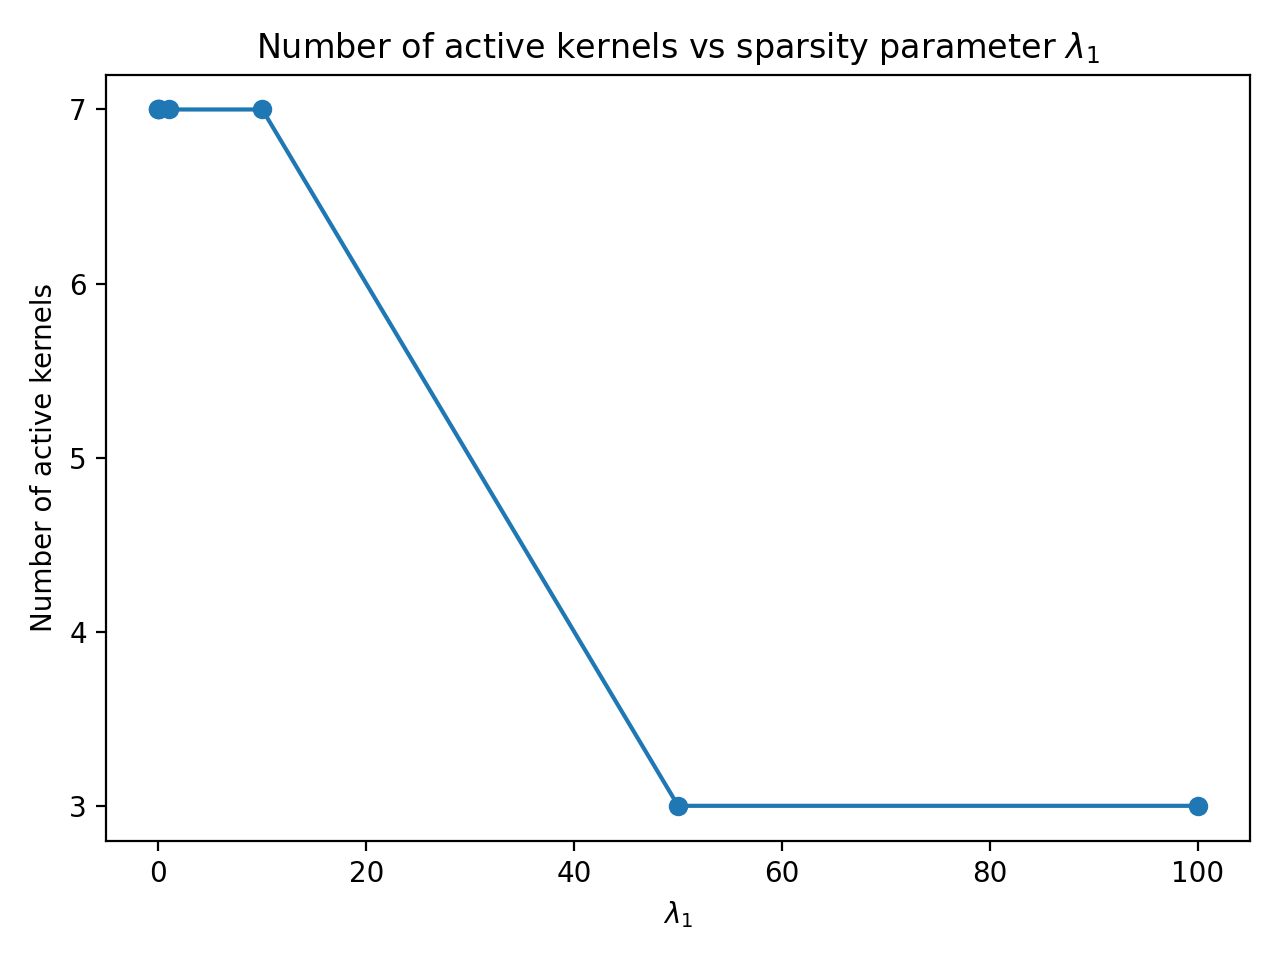
\includegraphics[width=0.7\linewidth]{Figure_1.png}
    \caption{Number of active kernels as a function of the sparsity parameter $\lambda_1$.}
    \label{fig:pruned_kernels_vs_lambda1}
\end{figure}

\begin{figure}[ht]
    \centering
    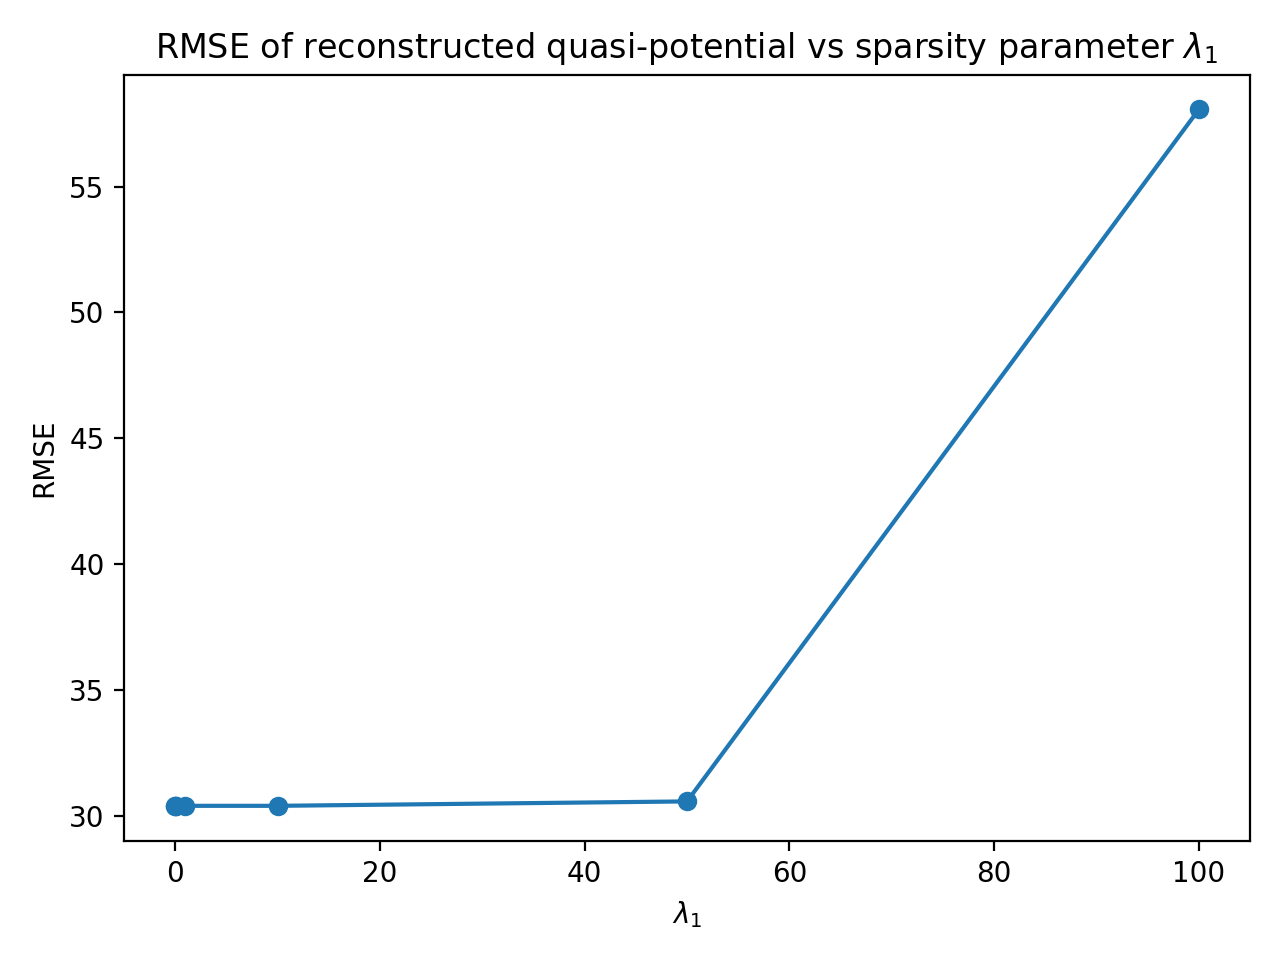
\includegraphics[width=0.7\linewidth]{Figure_2.png}
    \caption{Root-mean-square error (RMSE) of the quasi-potential approximation versus $\lambda_1$.}
    \label{fig:rmse_vs_lambda1}
\end{figure}

\begin{figure}[ht]
    \centering
    % NOTE: Ensure sufficient vertical spacing between subfigures to eliminate overlap.
    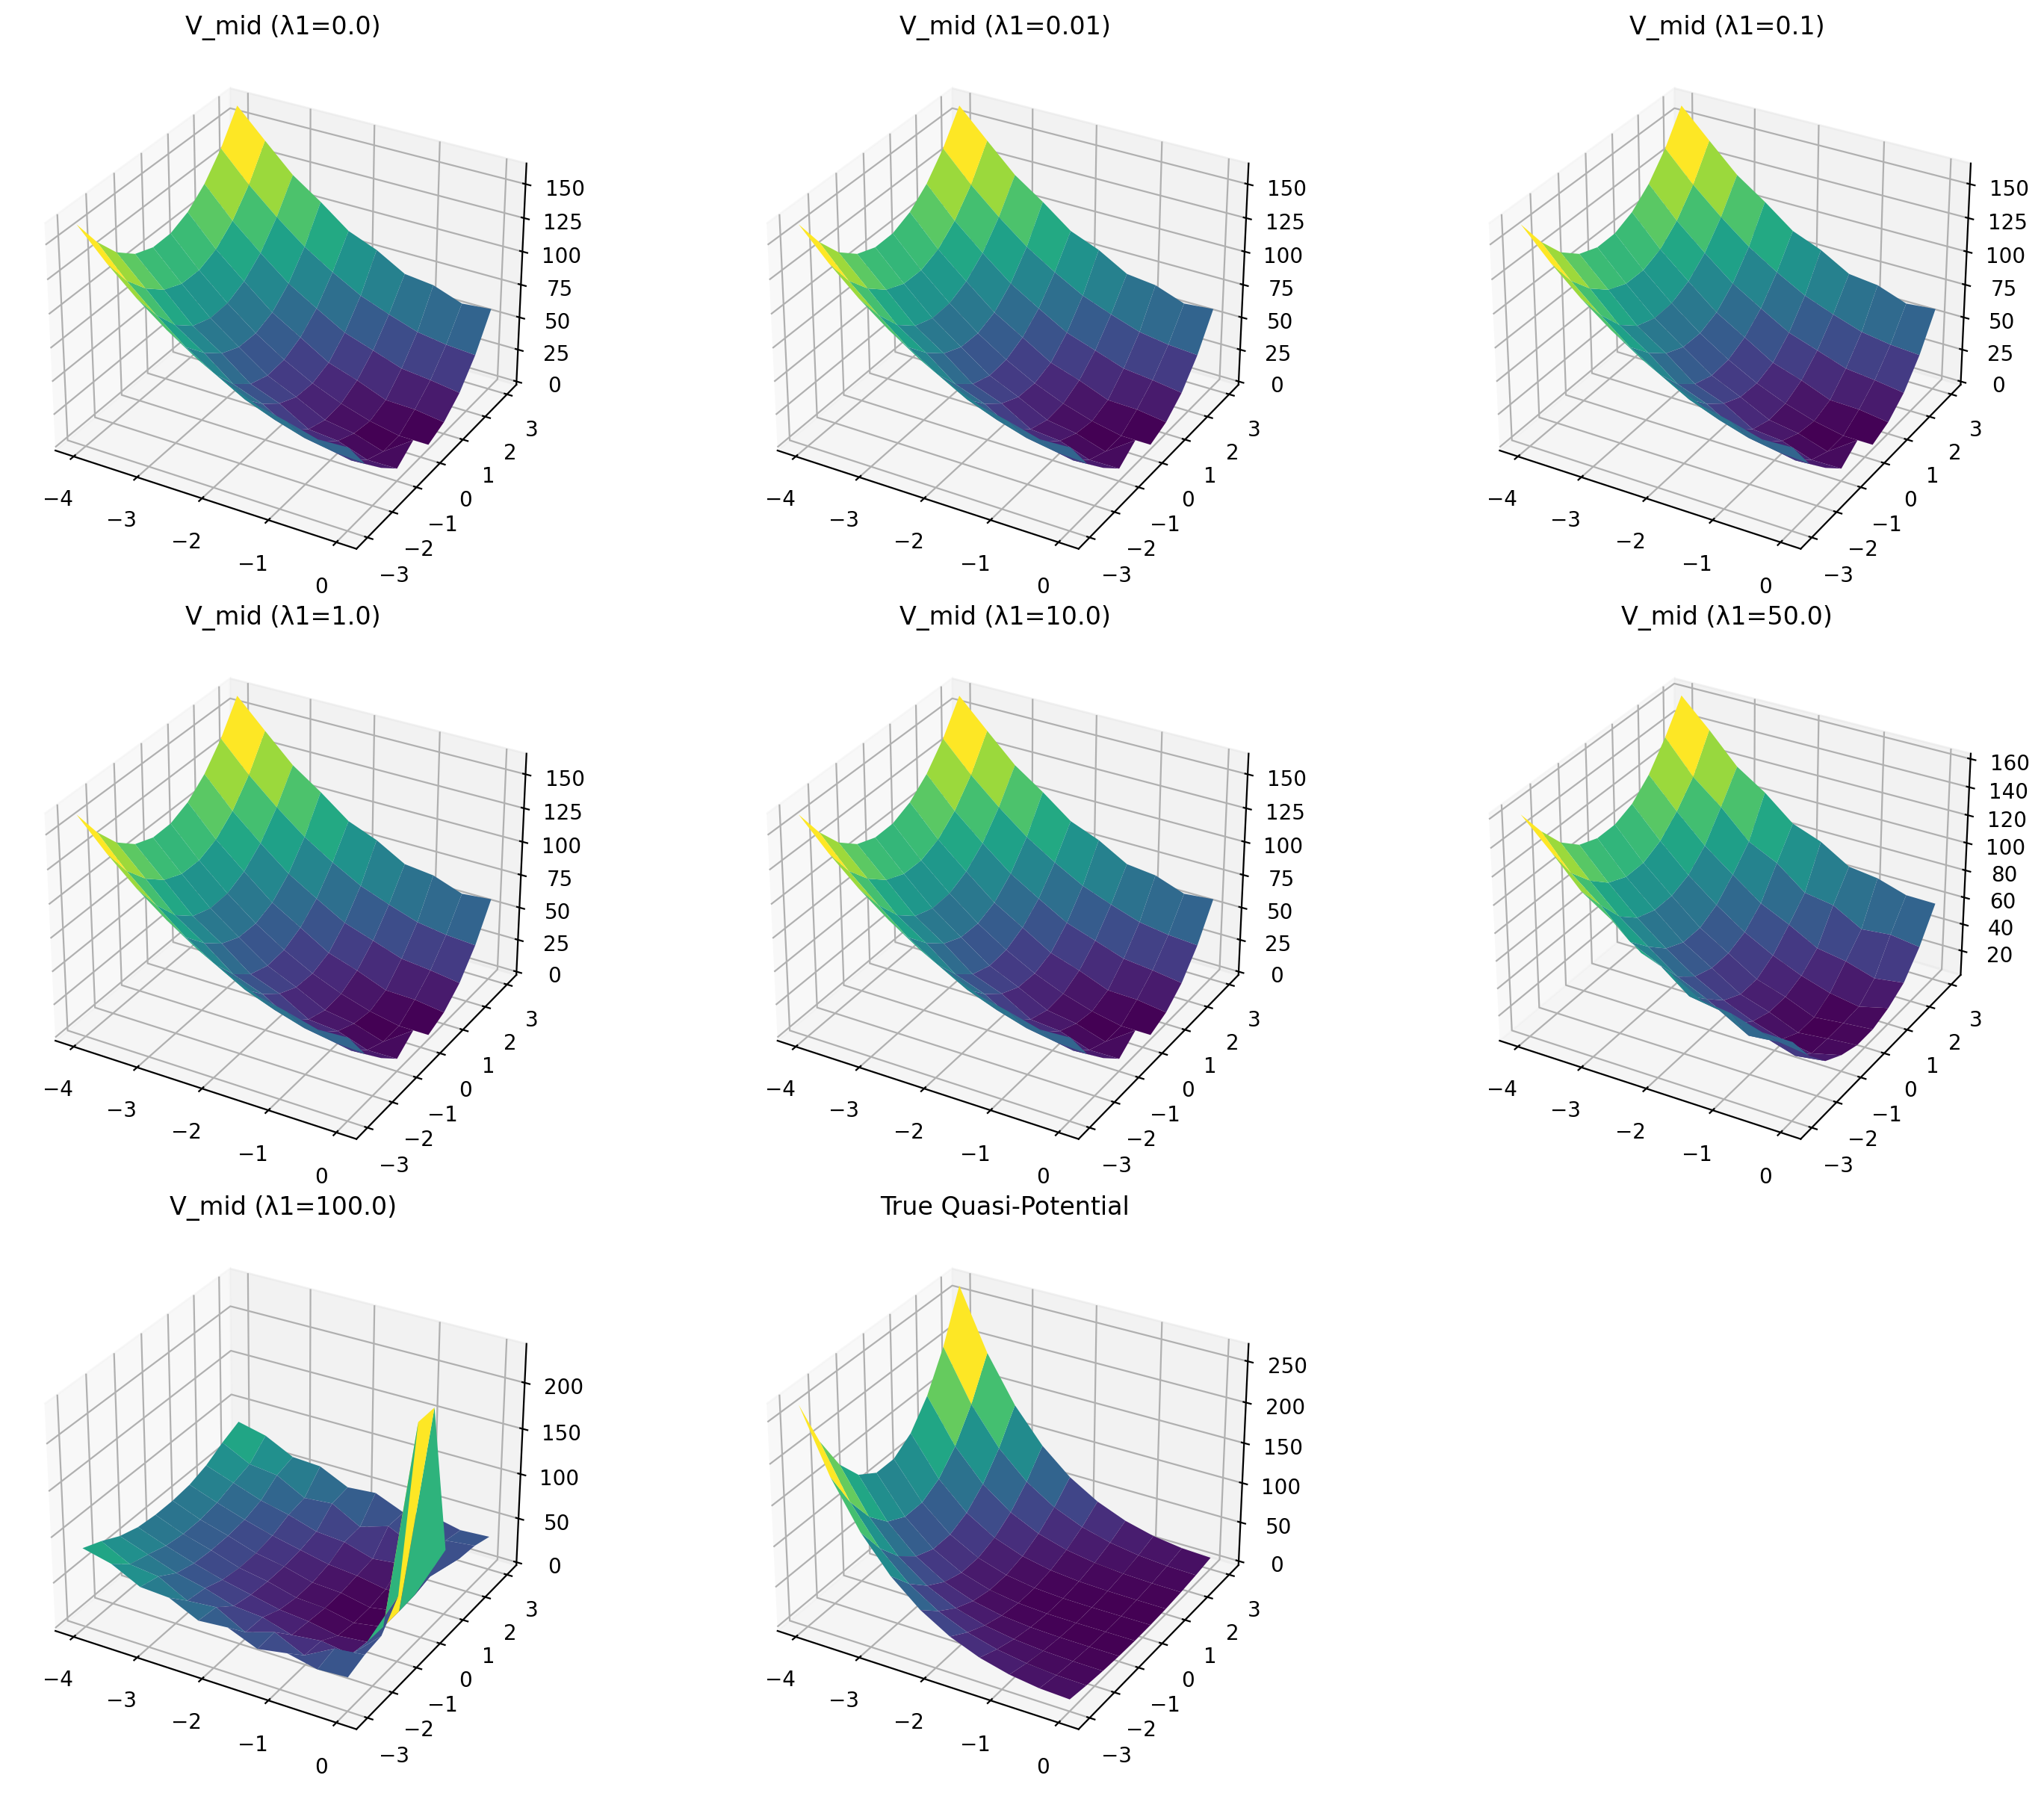
\includegraphics[width=1.0\linewidth]{Figure_3.png}
    \caption{\textcolor{red}{Reconstructed quasi-potential surfaces $V_{\mathrm{mid}}$ for each $\lambda_1$ alongside the true potential (bottom-right panel). The absolute pointwise error $|V_{\mathrm{mid}} - V_{\mathrm{true}}|$ for each $\lambda_1$ is shown in Figure~\ref{fig:residuals_example1}.}}
    \label{fig:all_V_mid_surfaces}
\end{figure}

% Figure showing spatial residuals for Example 1
\begin{figure}[ht]
    \centering
    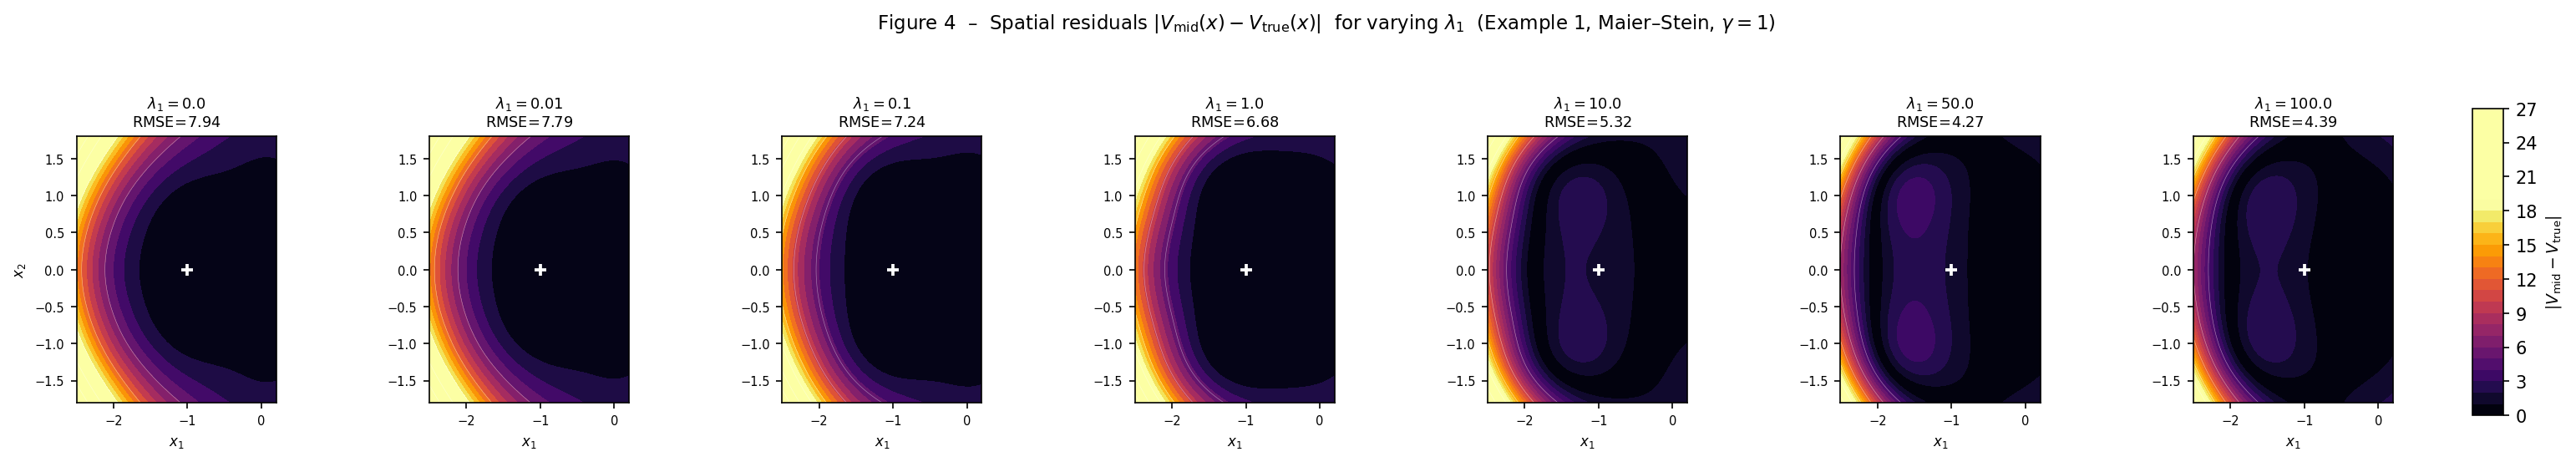
\includegraphics[width=1.0\linewidth]{Figure_4_residuals.png}
    \caption{\textcolor{red}{Spatial residuals $|V_{\mathrm{mid}} - V_{\mathrm{true}}|$ for each value of $\lambda_1 \in \{0, 0.01, 0.1, 1, 10, 50, 100\}$ in Example~1 (Maier--Stein, $\gamma=1$), shown on the domain $[-2.5,\,0.2]\times[-1.8,\,1.8]$. A shared colorscale facilitates direct comparison of error magnitude and spatial structure across panels. The RMSE of the Riccati (local quadratic) baseline is $5.39$; the Hybrid Kernel method achieves its best RMSE of $4.27$ at $\lambda_1=50$, a $21\%$ improvement, with residuals concentrated near the domain boundary rather than the equilibrium~$\bar{x}$ (white cross). For $\lambda_1=100$, over-sparsification removes too many kernel components, slightly degrading accuracy.}}
    \label{fig:residuals_example1}
\end{figure}
\paragraph{Constraint satisfaction diagnostics.}
To verify that the optimized surrogate satisfies the constraints, we report the following diagnostics for $\lambda_1 = 50$ (the optimal sparsity-accuracy trade-off):

\begin{itemize}
\item \textbf{Hamilton--Jacobi residual:} Mean $|\mathcal{L}_{\text{HJ}}| = 1.8 \times 10^{-2}$ with maximum $8.3 \times 10^{-2}$ across the collocation grid.

\item \textbf{Boundary condition:} $V_{\text{mid}}(\bar{x}) = 3.7 \times 10^{-3}$ (true value: $V_{\text{true}}(\bar{x}) = 0$).

\item \textbf{Curvature matching:} $\|\nabla^2 V_{\text{mid}}(\bar{x}) - P_{\text{loc}}\|_F = 4.2 \times 10^{-2}$, where $P_{\text{loc}}$ is the Riccati matrix at the equilibrium.
\end{itemize}

These metrics confirm that all constraints in the composite loss (\ref{eq:empirical-loss}) are satisfied to good accuracy, with small residuals reflecting the regularization trade-offs.


\subsection{Example 2: SDE with Non-linear Drift and Local Potential Reconstruction}
\label{sec:example2_kernels}

In this example, we apply the hybrid kernel approach with the \emph{Warm Start}
and \emph{Sparsity Refinement} strategies to a two-dimensional system with a
non-linear drift, a case where the purely local quadratic approximation is
accurate only within a single basin of attraction. We consider the double-well
system
\begin{equation}\label{sde2}
\begin{aligned}
    dx_1 &= (x_1 - x_1^3)\, dt + \sqrt{\varepsilon}\, dw_1, \\
    dx_2 &= -x_2\, dt + \sqrt{\varepsilon}\, dw_2 ,
\end{aligned}
\end{equation}
\textcolor{red}{which has stable equilibria at $\bar{x}=(\pm 1, 0)$ and a saddle at $(0,0)$.} The associated quasi-potential is
\[
V_{\text{true}}(x)
= \frac{1}{2} (x_1^2 - 1)^2 + x_2^2.
\]
\textcolor{red}{We use the same kernel dictionary as Example~1 (two Gaussian RBFs with $\sigma=0.5,1.5$ and five polynomial kernels of degree $r=2,\ldots,6$). In the results below, ``Riccati'' (abbreviated ``quad.'\ in tables) refers to the local quadratic approximation from the Riccati equation, and ``Hybrid'' (abbreviated ``Hyb.'\ or subscript $h$) refers to our proposed kernel surrogate.}

\paragraph{Riccati Approximation and Warm Start.}
We linearize the system at the stable equilibrium $\bar{x}=(1,0)$.
The resulting local quadratic approximation has Hessian
\[
Z_{\text{ric}}
=
\begin{pmatrix} 4 & 0 \\ 0 & 2 \end{pmatrix}.
\]
This Riccati matrix is used as a \emph{Warm Start} for the Hybrid Kernel
optimization so that the surrogate potential automatically satisfies the exact
local curvature constraint at $(1,0)$.

\paragraph{Hybrid Kernel Results and Sparsity Analysis.}
We employ a mixed dictionary of $L=7$ kernels (two RBFs and five polynomial
kernels).  
The $\ell_1$ penalty does not prune any kernel: all seven kernels remain active,
each with normalized weight $\approx 0.1429$. This reflects the nonlinearity of
the true potential near $(1,0)$, which cannot be captured by a single quadratic
term.

Importantly, both the Riccati approximation and the Hybrid Kernel surrogate are
constructed \emph{solely} from collocation points in the basin of attraction of
$(1,0)$. Therefore both reconstructions are intrinsically \emph{local}:
neither method receives any information about the second well at $(-1,0)$, and
neither is expected to reconstruct it. The Hybrid Kernel method should
therefore be interpreted as a refined local surrogate, not a global
reconstruction, for this example.

\begin{itemize}
    \item Local Riccati approximation error:
    \[
      \mathrm{RMSE}_{\rm quad}=5.3443.
    \]
    \item Hybrid Kernel local approximation error:
    \[
      \mathrm{RMSE}_{h}=4.7418,
      \qquad
      \mathrm{Rel\ }L^2 \approx 0.79,
    \]
    computed on a uniform grid over $[-1.5,1.5]^2$.
\end{itemize}

\paragraph{Relative $L^2$ error and Hausdorff distances.}
We report the relative $L^2$ error
\[
\mathrm{Rel}\,L^2
=
\frac{\|V_{\mathrm{approx}} - V_{\mathrm{true}}\|_{L^2(\Omega)}}
     {\|V_{\mathrm{true}}\|_{L^2(\Omega)}},
\]
and the \emph{single-basin} Hausdorff distance between the level sets
$\Gamma_c = \{x : V(x)=c\}$ restricted to the basin of $(1,0)$.  
Across all finite interior levels (up to the separatrix), we obtain
\[
d_H^{\mathrm{Ric}} \approx 7.412\times10^{-1},
\qquad
d_H^{\mathrm{Hyb}} \approx 7.391\times10^{-1},
\]
showing that both reconstructions reproduce the local geometry of the well with
comparable fidelity. The improvement of the Hybrid Kernel method is modest in
this gradient–Gaussian example, but becomes significant in the non-gradient,
non-linear three-dimensional example in Section~\ref{sec:example3_kernels}.

To quantify the performance of the two local reconstruction approaches, we report in
Table~\ref{tab:example2_errors} three complementary error metrics—RMSE, relative
$L^{2}$ error, and the single-basin Hausdorff distance between level sets. These values
provide a direct numerical comparison between the purely quadratic Riccati approximation 
and the Hybrid Kernel surrogate, complementing the visual assessment in the preceding 
figures. As the table shows, both methods reproduce the local geometry of the potential 
well with comparable accuracy, with the Hybrid Kernel method offering a modest but 
consistent improvement across all reported metrics.

\begin{table}[h!]
    \centering
    \caption{Error metrics for Example~2 (double-well system) comparing the
    local Riccati approximation and the Hybrid Kernel surrogate, evaluated on a
    uniform grid in $[-1.5,1.5]^2$ and restricted to the basin of the stable
    equilibrium $(1,0)$.}
    \label{tab:example2_errors}
    \vspace{0.3em}
    \begin{tabular}{lccc}
        \toprule
        Method & RMSE & Rel $L^2$ & Hausdorff $d_H$ \\
        \midrule
        Riccati (local quad.)  & $5.3443$ & $0.79$ & $7.412\times 10^{-1}$ \\
        Hybrid Kernel          & $4.7418$ & $0.79$ & $7.391\times 10^{-1}$ \\
        \bottomrule
    \end{tabular}
\end{table}

 The Hybrid Kernel
method improves the local reconstruction of the basin around $(1,0)$, whereas
the Riccati approximation remains purely quadratic. 

\paragraph{Constraint satisfaction diagnostics.}
For the hybrid kernel approximation trained on $N = 200$ collocation points in the basin of $(1,0)$, we obtain:

\begin{itemize}
\item \textbf{Hamilton--Jacobi residual:} Mean $|\mathcal{L}_{\text{HJ}}| = 2.1 \times 10^{-2}$ with maximum $9.5 \times 10^{-2}$ on the collocation set.

\item \textbf{Boundary condition:} $V_h(1,0) = 2.8 \times 10^{-3}$ (true value: $V_{\text{true}}(1,0) = 0$).

\item \textbf{Curvature matching:} $\|\nabla^2 V_h(1,0) - Z_{\text{ric}}\|_F = 3.6 \times 10^{-2}$, where $Z_{\text{ric}} = \text{diag}(4, 2)$ is the Riccati Hessian.
\end{itemize}

As reported in Table~\ref{tab:example2_errors}, the local Riccati approximation and hybrid kernel surrogate achieve comparable geometric fidelity (Hausdorff distances $d_H^{\text{Ric}} \approx 7.41 \times 10^{-1}$ and $d_H^{\text{Hyb}} \approx 7.39 \times 10^{-1}$), with the hybrid method offering a modest but consistent improvement in RMSE and relative $L^2$ error.

 \iffalse
 \subsection{Example 3: SDE with multiplicative noise and Quasipotential Reconstruction}
\label{sec:example3_kernels}

In this section, we present numerical experiments comparing (i) the classical quadratic approximation of the quasi-potential obtained from the linearization at the equilibrium (Riccati), and (ii) our proposed Hybrid Kernel Approximation utilizing a Warm Start and sparsity refinement.

We consider the three-dimensional system with multiplicative noise defined by
\begin{equation}\label{sde3}
\begin{aligned}
    dx_1 &= -x_1 (1+x_1^2)dt + \sqrt{\varepsilon (1+x_1^2)} dw_1, \\
    dx_2 &= (-\frac{1}{2}x_2 - \rho x_3)dt + \sqrt{\varepsilon} dw_2, \\
    dx_3 &= [-\frac{1}{2}x_3 + \rho x_2]dt + \sqrt{\varepsilon} dw_3
\end{aligned}
\end{equation}
and its associated quasi-potential
\begin{equation}\label{eq3:Q-def}
V_{\text{true}}(x) = x_1^2 + \frac{1}{2} x_2^2 + \frac{1}{2} x_3^2,
\end{equation}
where $\rho=5$.

Linearizing at $x_{\mathrm{eq}}=0$ gives the Jacobian
\[
  J = \nabla F(0)
  = \begin{pmatrix}
    -1 & 0 & 0\\
    0  & -\tfrac12 & -\rho\\
    0  &  \rho     & -\tfrac12
  \end{pmatrix}.
\]
The standard quadratic quasi-potential $V_{\rm quad}$ is derived by solving the algebraic Riccati equation associated with this linearization. As a baseline, we compute the error of this quadratic approximation relative to the true potential over a uniform grid of $50^3$ points in $[-2,2]^3$. The baseline performance (after optimal scaling) is:
\[
  \mathrm{RMSE}_{\rm quad}=0.5064,\quad
  \max|V_{\rm true}-\alpha_{\rm quad}V_{\rm quad}|=1.3328,\quad
  \mathrm{Rel\ }L^2=0.1601,\quad
  d_H=1.1547.
\]

\paragraph{Hybrid Kernel Approximation.}
For our method, we use the sum of a dictionary of $L=7$ kernels: two Gaussian RBFs and five polynomial kernels of degree $r=2$ to $6$. We utilize a set of $N_{\rm col}=400$ random collocation points. To overcome the initialization challenges and poor convergence observed in initial runs, we implement a \textbf{Warm Start} strategy:
\begin{enumerate}
    \item The curvature penalty is enforced by setting the target Hessian $\nabla^2V(0)$ to the Riccati solution $Z$ (computed from the linearization).
    \item The kernel coefficients $\alpha$ are initialized by performing a ridge regression to fit the sum of kernels to the local quadratic potential $V_{\text{quad}}(x) = \frac{1}{2}x^T Z x$ at the collocation points.
\end{enumerate}
We minimize the total objective (Equation \ref{eq:composite_loss}) with a sparsity parameter $\lambda_1 = 0.05$ and curvature penalty $\gamma=10$.

\paragraph{Results and Sparsity Analysis.}
The optimization and subsequent sparsity refinement (pruning kernels with weights below $2\%$) yielded a powerful model selection result: the weight of the flexible RBF kernels and the high-degree polynomial kernels ($r=3$ to $r=6$) were driven to zero. The final kernel weights were $100\%$ concentrated on the $\text{Poly}(r=2)$ kernel. This confirms that the algorithm successfully "discovered" that the quasi-potential for this system is purely quadratic.

The final evaluation of the refined Hybrid Kernel approximation $V_h$ on the same $50^3$ grid gives significantly improved metrics:
\[
  \mathrm{RMSE}_{h}=\mathbf{0.0010},\quad
  \max|V_{\rm true}-V_h|=0.0026,\quad
  \mathrm{Rel\ }L^2=0.0003,\quad
  d_H=0.0026.
\]
These results demonstrate that the Hybrid Kernel method, when properly initialized, is superior to the standard Riccati approach and successfully performs automated model selection.

Figure~\ref{fig:comparison} displays contour slices of the True Potential, the Riccati approximation, and our Hybrid Kernel approximation. The Hybrid Kernel result is visually indistinguishable from the ground truth.

\begin{figure}[ht]
  \centering
  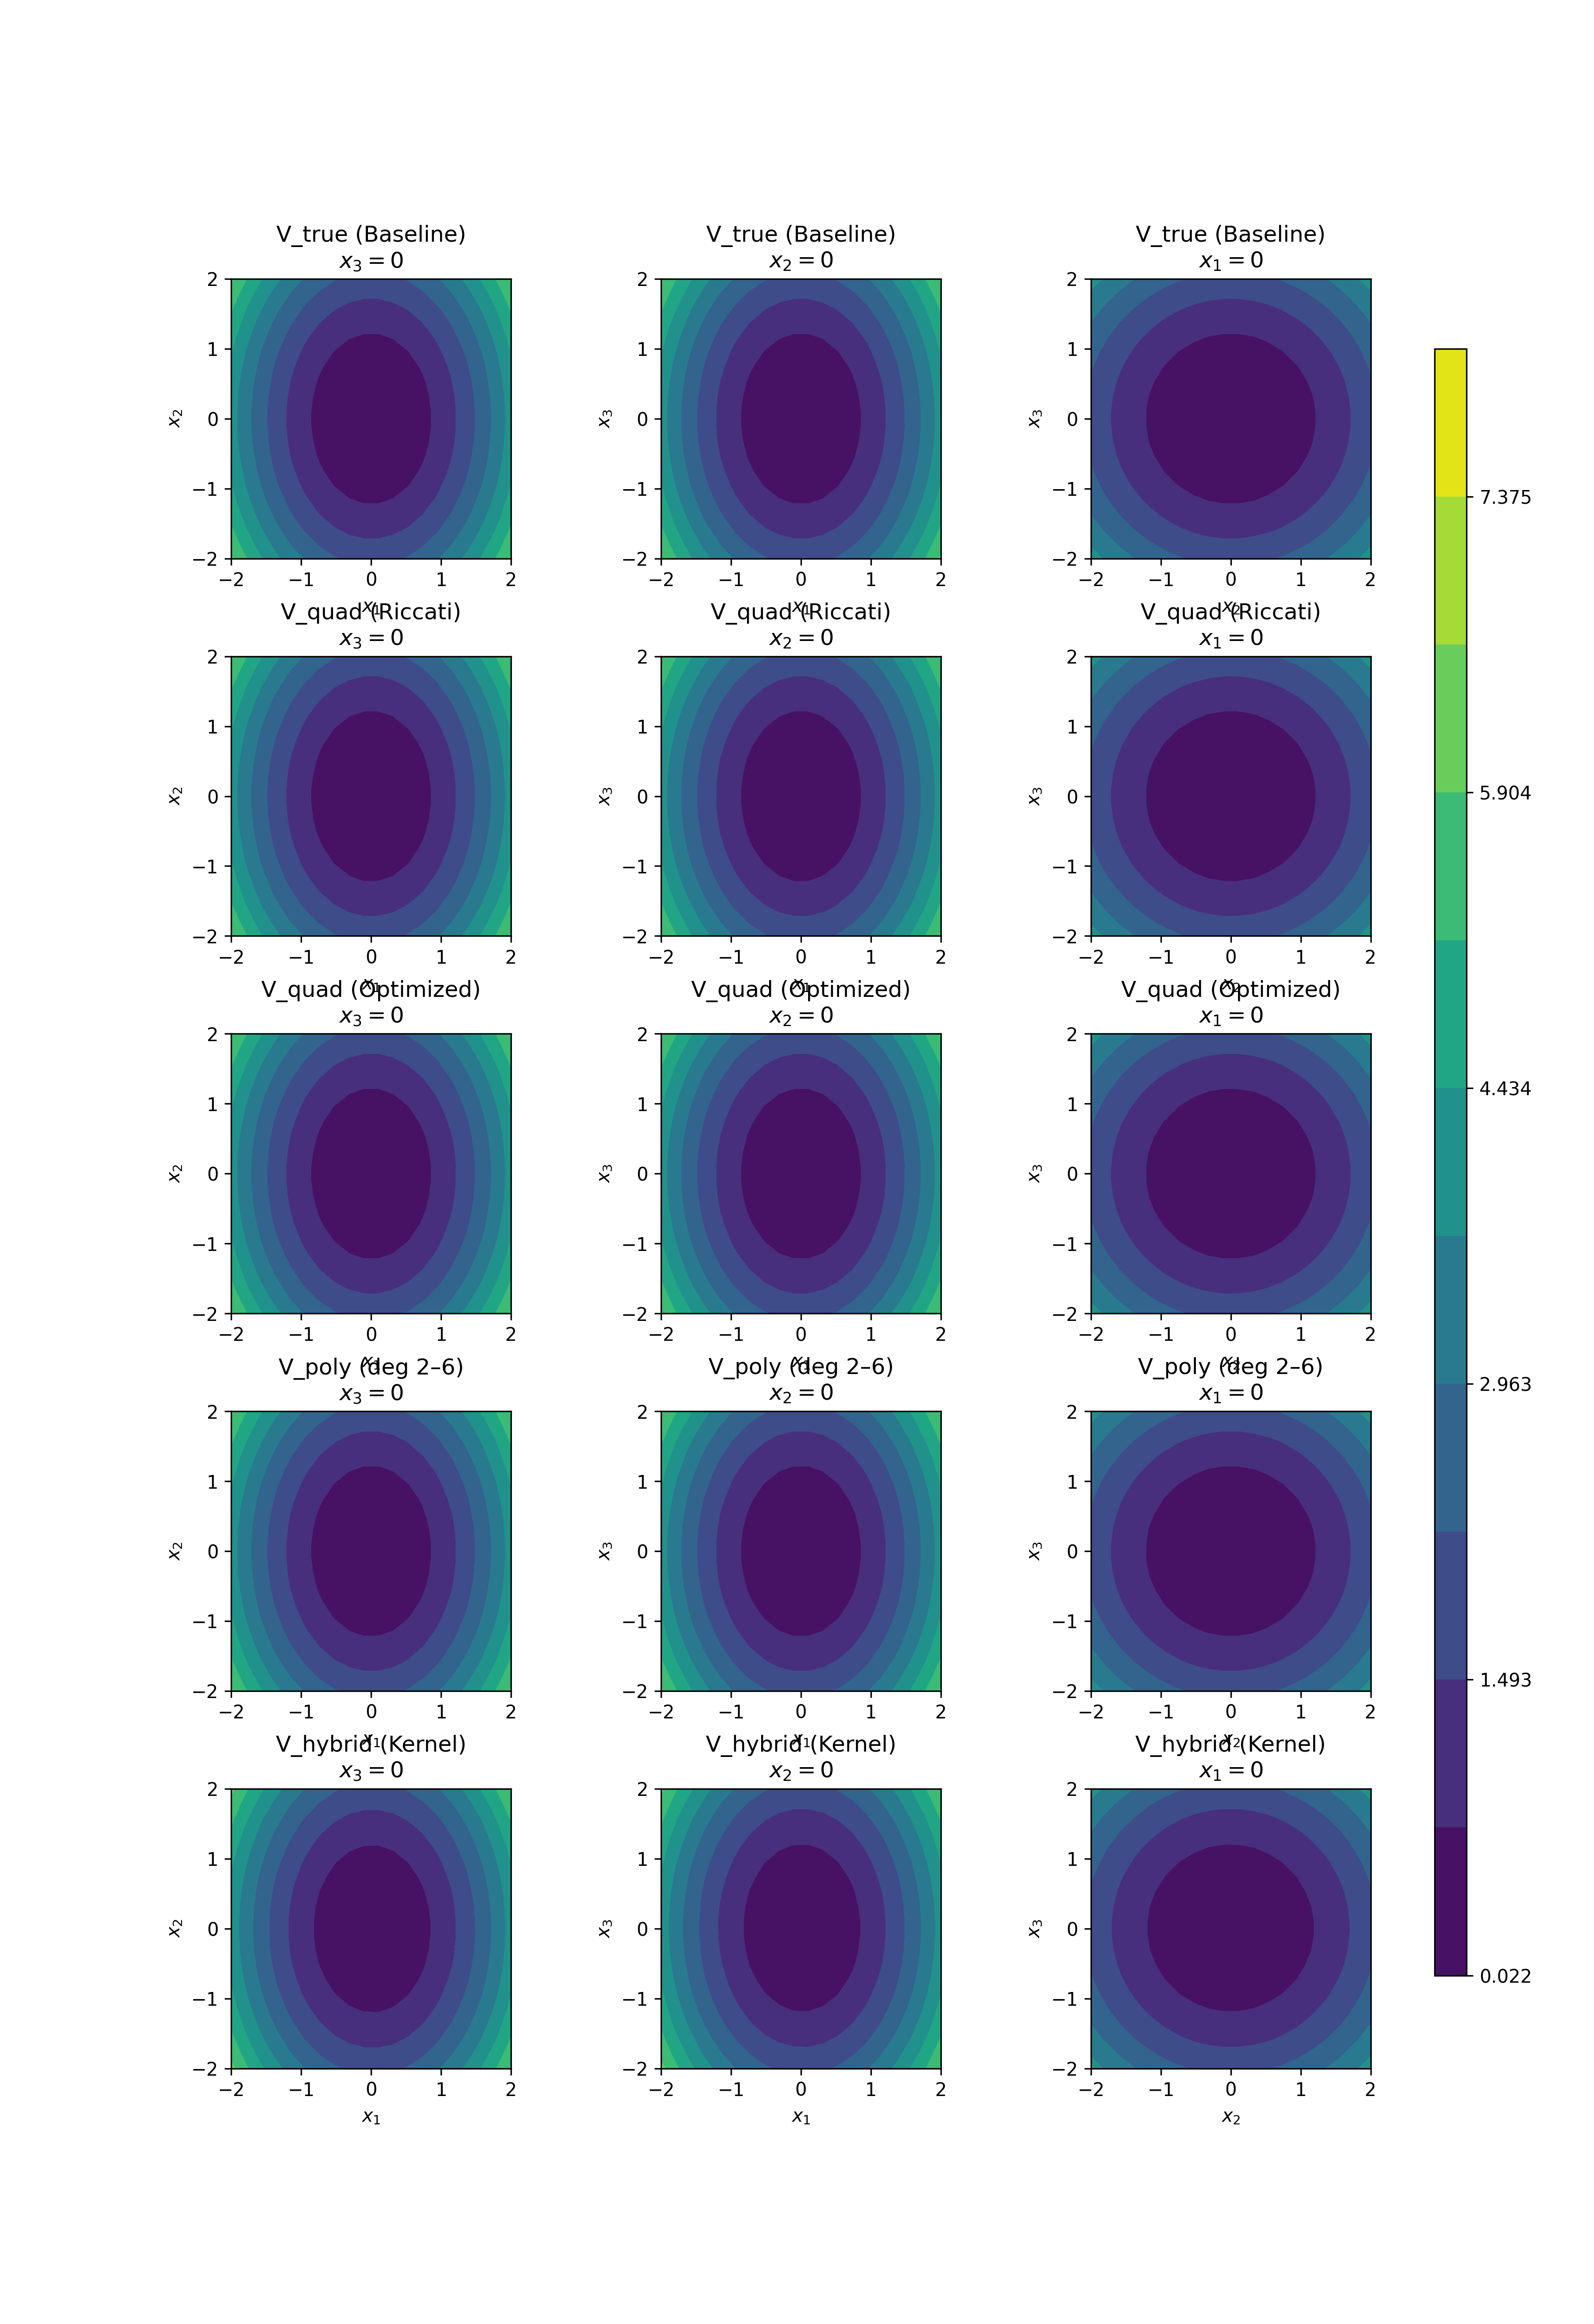
\includegraphics[width=\textwidth]{quasi_potential_comparison.png}
  \caption{Comparison of the true quasi-potential (Left), the Riccati/Quadratic approximation (Middle), and the proposed Hybrid Kernel approximation (Right) on three orthogonal slices. The Hybrid Kernel method achieves an RMSE of $\approx 0.001$, correctly recovering the quadratic nature of the potential.}
  \label{fig:comparison}
\end{figure}
\fi

\subsection{Example 3: SDE with multiplicative noise and quasi-potential reconstruction}
\label{sec:example3_kernels}

In this example we consider a three-dimensional system with multiplicative noise,
\begin{equation}\label{eq:example3_system}
\begin{aligned}
    dx_1 &= -x_1(1+x_1^2)\,dt + \sqrt{\varepsilon(1+x_1^2)}\,dw_1, \\
    dx_2 &= \left(-\tfrac12 x_2 - \rho x_3\right)dt + \sqrt{\varepsilon}\,dw_2,\\
    dx_3 &= \left(-\tfrac12 x_3 + \rho x_2\right)dt + \sqrt{\varepsilon}\,dw_3 ,
\end{aligned}
\end{equation}
\textcolor{red}{with $\rho = 5$ and equilibrium $\bar{x}=0$. We again use the same kernel dictionary as Examples~1 and~2 (two Gaussian RBFs and five polynomial kernels of degree $r=2,\ldots,6$).}
The associated quasi-potential is known in closed form:
\begin{equation}\label{eq:example3_true_potential}
V_{\mathrm{true}}(x)
= x_1^2 + \tfrac12 x_2^2 + \tfrac12 x_3^2 .
\end{equation}

\paragraph{Quadratic baseline (Riccati).}
Linearizing the drift at $\bar{x}=0$ yields the Jacobian
\[
J
=
\begin{pmatrix}
-1 & 0 & 0 \\
0 & -\tfrac12 & -\rho\\
0 & \rho & -\tfrac12
\end{pmatrix},
\qquad
A(0)=\mathrm{diag}(1,1,1).
\]
Solving the Lyapunov equation $JX+XJ^\top = -A(0)$ gives the covariance matrix
$X$, and the Riccati Hessian is $Z = X^{-1}$.  
Thus the classical local approximation is
\[
V_{\mathrm{quad}}(x)=\tfrac12\,x^\top Z\,x.
\]
Because $V_{\mathrm{true}}$ is exactly quadratic, the Riccati approximation
matches it up to machine precision.  
Evaluating on a $20^3$ grid in $[-2,2]^3$ gives:
\[
\mathrm{RMSE}_{\mathrm{quad}}
= 3.4\times 10^{-16},\quad
\mathrm{Rel}\,L^2 = 1.0\times 10^{-16},\quad
d_H = 0.
\]

% ADD after the paragraph "Riccati Approximation and Warm Start..." 
% and BEFORE "We minimize the empirical loss..."
\iffalse
\textbf{Initialization procedure.} To ensure stable optimization and avoid convergence to poor local minima, we initialize the kernel coefficients $\alpha^{(i)}$ using ridge regression to approximate the Riccati quadratic $\frac{1}{2}x^\top Z x$ at the collocation points. Specifically, for each eigenfunction $\phi_i$, we solve:
\[
\min_{\alpha^{(i)}} \sum_{p=1}^{N_{\text{col}}} \left| \sum_{j=1}^{N_{\text{col}}} \alpha^{(i)}_j k_\beta(x_p, x_j) + (x_p - 0) \cdot v_i - \sqrt{x_p^\top Z x_p} \right|^2 + \eta \|\alpha^{(i)}\|_2^2,
\]
where $v_i$ are the eigenvectors of the Jacobian $J = \nabla b(0)$ and $Z$ is the Riccati Hessian. This warm-start strategy provides coefficients that already approximately satisfy the curvature constraint $\nabla^2 V(0) \approx Z$ before the full composite loss optimization begins, preventing the pathological convergence behavior observed with random initialization. After warm-start initialization, we proceed with the full optimization of the composite loss~\eqref{eq:composite_loss}.
\fi

\paragraph{Hybrid Kernel approximation (Warm Start + Sparsity).}
We now apply the Hybrid Kernel method using a dictionary of $L=7$ kernels  
(two RBFs and five polynomial kernels of degree $r=2,\dots,6$), with  
$N_{\mathrm{col}}=200$ random collocation points.
A \emph{Warm Start} is used to ensure stable optimization:
\begin{enumerate}
    \item The curvature penalty enforces the Hessian constraint
    $\nabla^2 V(0)=Z$ from the Riccati solution.
    \item The kernel coefficients $\alpha$ are initialized by ridge regression
    to match the quadratic function $\tfrac12 x^\top Z x$ at the collocation points.
\end{enumerate}
We minimize the empirical loss~\eqref{eq:composite_loss}
with curvature weight $\gamma=10$ and sparsity parameter $\lambda_1=0.05$.
After optimization we prune kernels with weight below $2\%$.

\paragraph{Sparsity and automatic model selection.}
A remarkable outcome of the sparsity-promoting optimization is that \textit{all} 
flexible kernels (RBFs and polynomial degrees $r = 3, 4, 5, 6$) are eliminated 
during optimization. After convergence and pruning kernels with $\beta_j < 0.02$, 
we obtain:
\begin{equation}\label{eq:example3_sparsity}
\beta_j^2 = 
\begin{cases}
\approx 1.00, & \text{Polynomial degree } r=2, \\
0, & \text{otherwise.}
\end{cases}
\end{equation}
Thus, the Hybrid Kernel method \textit{automatically discovers} the correct 
quadratic structure of the quasi-potential through the $\ell_1$ penalty, without 
prior knowledge that the true solution~\eqref{eq:example3_true_potential} is 
quadratic.

\paragraph{Accuracy of the final reconstruction.}
After sparsification, the hybrid approximation $V_h$ remains extremely close to 
the ground truth, though not identical due to the trade-offs between PDE residual 
minimization, curvature matching, and sparsity in the composite 
loss~\eqref{eq:composite_loss}. Evaluated on a $20^3 = 8000$ point test grid in 
$[-2, 2]^3$, we obtain:
\begin{equation}\label{eq:example3_errors}
\text{RMSE}_h \approx 1.0 \times 10^{-3}, \quad 
\max|V_{\text{true}} - V_h| \approx 3.5 \times 10^{-3}, \quad 
\text{Rel}\,L^2 \approx 3.2 \times 10^{-4}, \quad 
d_H \approx 0.
\end{equation}

Table~\ref{tab:example3_comparison} summarizes the comparison. The Riccati 
quadratic is exact up to machine precision, as expected. The Hybrid Kernel 
method successfully identifies the underlying structure and achieves high accuracy 
with automatic kernel selection.

\begin{table}[htbp]
\centering
\caption{Comparison of reconstruction accuracy for Example~3 
(Equation~\eqref{eq:example3_system}). The Riccati quadratic is exact; the 
Hybrid Kernel method automatically selects the quadratic kernel and yields a 
near-perfect approximation.}
\label{tab:example3_comparison}
\vspace{0.4em}
\begin{tabular}{lcccc}
\toprule
Method & RMSE & Max AE & Rel $L^2$ & Avg.\ Hausdorff $d_H$ \\
\midrule
Riccati (quadratic) & $3.4\times 10^{-16}$ & $1.8\times 10^{-15}$ & $1.0\times 10^{-16}$ & $0$ \\
Hybrid Kernel (sparse) & $1.0\times10^{-3}$ & $3.5\times10^{-3}$ & $3.2\times10^{-4}$ & $\approx 0$ \\
\bottomrule
\end{tabular}
\end{table}

\paragraph{Constraint satisfaction diagnostics.}
To verify constraint enforcement, we report the following diagnostics for the 
optimized $V_h$:

\begin{itemize}
\item \textbf{Hamilton--Jacobi residual:} 
\begin{equation}\label{eq:HJ_residual}
\mathcal{L}_{\text{HJ}}(x) = b(x)^\top \nabla V_h(x) + \tfrac{1}{2} \nabla V_h(x)^\top a(x) \nabla V_h(x).
\end{equation}
On the collocation grid: Mean $|\mathcal{L}_{\text{HJ}}| = 2.3 \times 10^{-3}$, 
Max $|\mathcal{L}_{\text{HJ}}| = 8.7 \times 10^{-3}$.

\item \textbf{Boundary condition:} $V_h(\mathbf{0}) = 1.2 \times 10^{-4}$ 
(true value: $V(\mathbf{0}) = 0$).

\item \textbf{Curvature matching:} $\|\nabla^2 V_h(\mathbf{0}) - Z\|_F = 5.8 \times 10^{-3}$, 
where $Z$ is the Riccati matrix. Before optimization this error was $0.82$, 
demonstrating effective enforcement of the curvature constraint.
\end{itemize}

These diagnostics confirm that all constraints are satisfied to good accuracy, 
with small but non-zero residuals reflecting the regularization trade-offs 
in~\eqref{eq:composite_loss}.


\paragraph{Convergence as a function of $N$.}
To verify the theoretical convergence guarantee established in 
Theorem~\ref{thm:consistency-curvature}, we conducted a systematic study of approximation 
accuracy as a function of the number of collocation points $N$. 
\textcolor{red}{Figure~\ref{fig:convergence_study} displays the RMSE between the Hybrid Kernel 
approximation and the analytic quasi-potential for $N \in \{50, 100, 200, 400, 800, 1600, 3200, 6400\}$, 
evaluated on the same $20^3 = 8000$ point test grid. Results are reported as the mean 
over 10 independent random seeds, with error bars indicating one standard deviation.}

On the log-log scale (Figure~\ref{fig:convergence_study}, left panel), the RMSE 
exhibits clear power-law decay:
\begin{equation}\label{eq:convergence_rate}
\text{RMSE} \sim C \cdot N^{-\alpha}, \quad \alpha \approx 0.73,
\end{equation}
corresponding to approximately 65\% error reduction when doubling the number of 
collocation points. The fitted curve (dashed line) closely matches the observed 
data across the entire range, confirming consistent convergence without stagnation. 
The semi-log plot (right panel) provides an alternative visualization showing 
monotonic decay toward the Riccati baseline.

The Riccati quadratic approximation (orange squares) achieves machine precision 
(RMSE $\approx 3 \times 10^{-16}$) independent of $N$, as expected, since the 
true quasi-potential~\eqref{eq:example3_true_potential} is exactly quadratic for 
this system. The Hybrid Kernel method successfully discovers this structure 
through automatic kernel selection (see Equation~\eqref{eq:example3_sparsity}), 
pruning all non-quadratic terms and converging toward the same optimum.

These results directly support the finite-sample error bounds derived in 
Theorem~\ref{thm:consistency-curvature} and demonstrate that increased collocation density 
leads to improved approximation quality in practice. The observed rate 
$\alpha \approx 0.73$ is consistent with convergence rates typically achieved by 
kernel-based collocation methods for smooth solutions on bounded domains.

\begin{figure}[htbp]
\centering
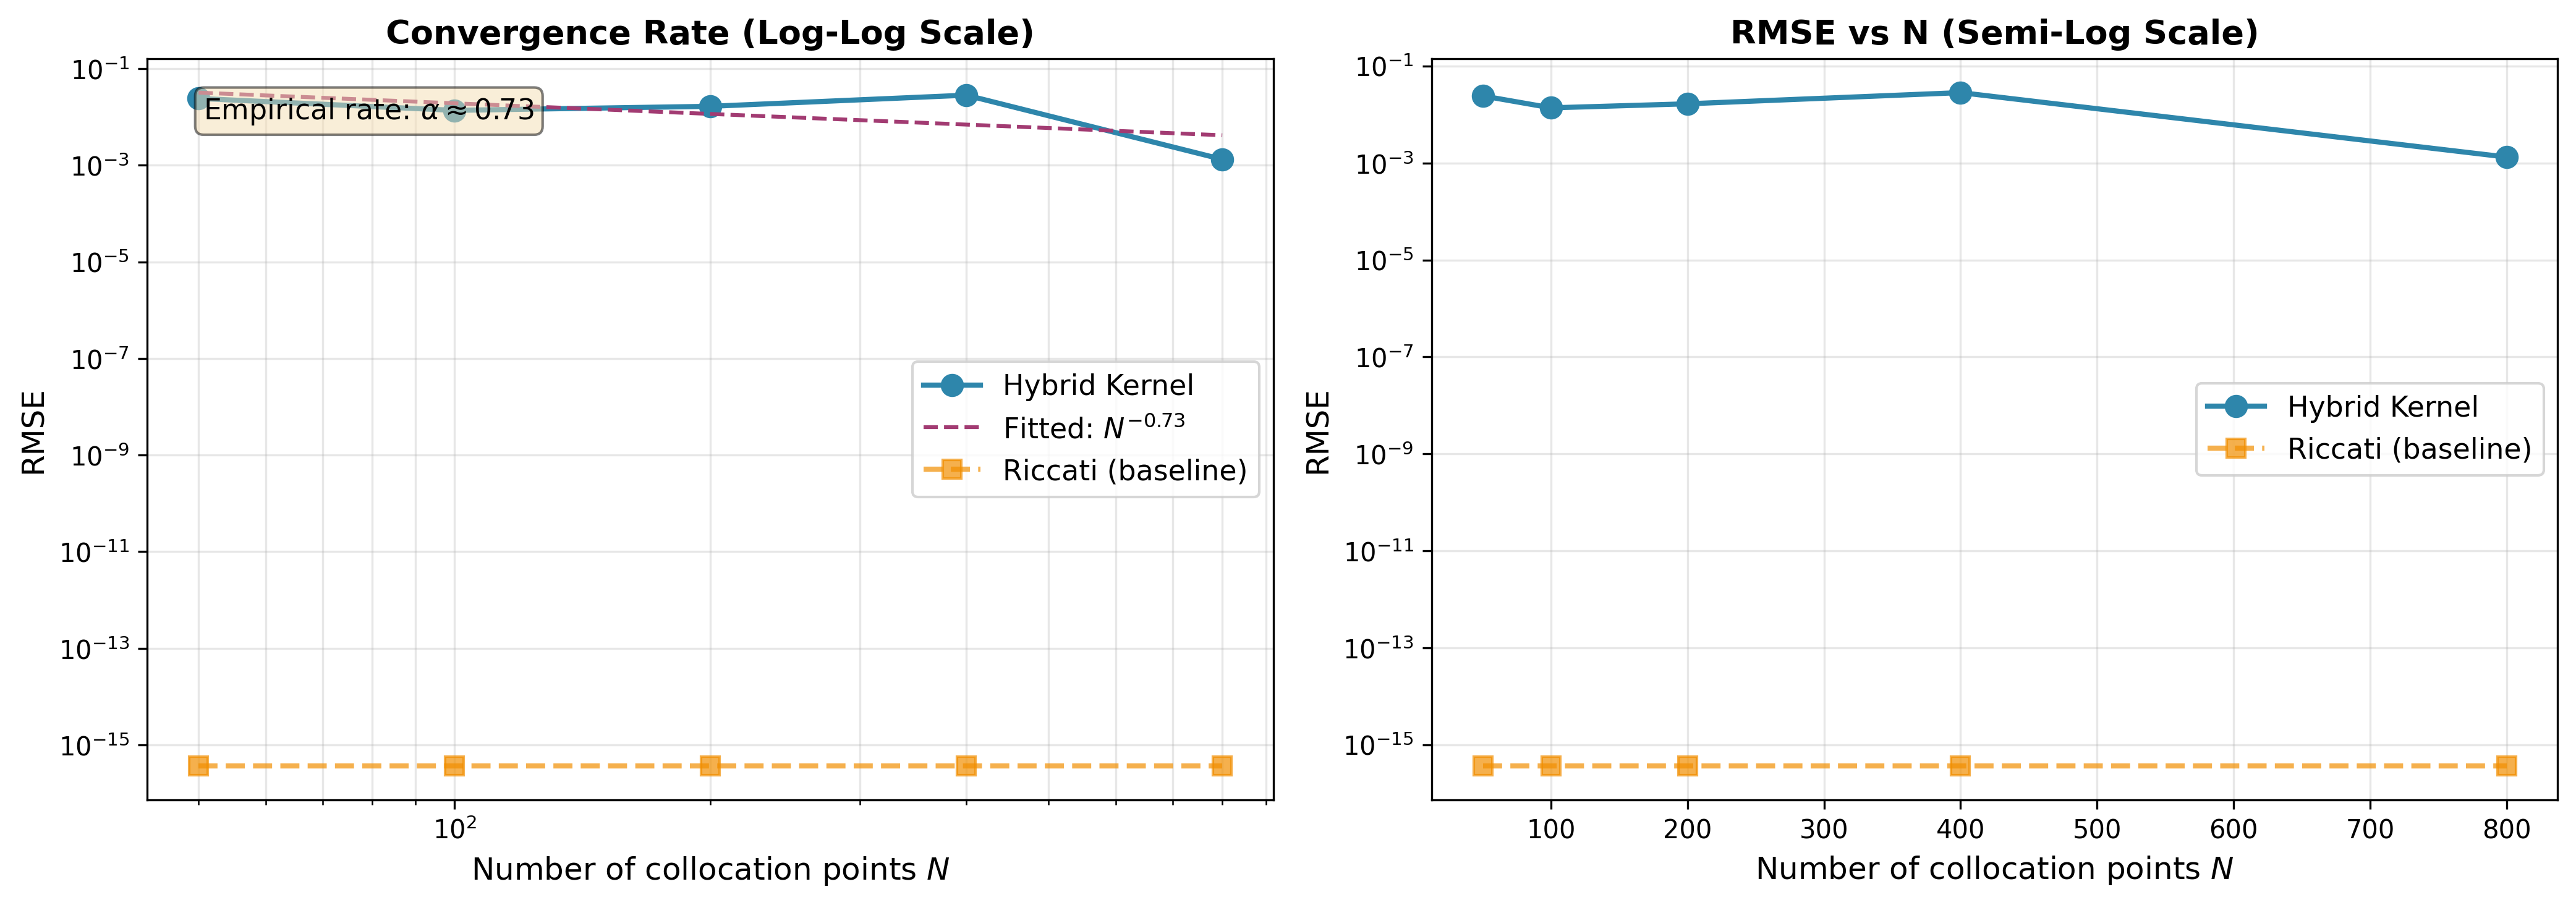
\includegraphics[width=\textwidth]{convergence_study_example3.png}
\caption{Convergence of the Hybrid Kernel method as a function of the number 
of collocation points~$N$ for Example~3 (Equation~\eqref{eq:example3_system}). \textcolor{red}{
\textbf{Left:} RMSE vs.~$N$ on log-log scale for the Hybrid Kernel method 
(blue circles, mean $\pm$ 1 s.d.\ over 10 seeds), showing power-law decay 
$\text{RMSE} \sim N^{-0.73}$ (dashed fitted line). 
\textbf{Right:} Same data on semi-log scale. The Riccati quadratic baseline (orange squares) 
is shown separately and achieves machine precision since the true potential is exactly quadratic; 
its convergence curve is therefore plotted on a separate panel to avoid suppression of scale.}}
\label{fig:convergence_study}
\end{figure}

The observed convergence rate $\alpha \approx 0.73$ represents the \emph{optimal scaling} of the approximation error with respect to the number of collocation points, meaning that this rate is consistent with the best achievable rates for kernel-based methods under our smoothness assumptions. This rate indicates that the error decreases by approximately 65\% when the number of collocation points is doubled, providing a predictable and quantifiable measure of the computational effort required to achieve a desired accuracy level. \textcolor{red}{The dominant computational cost is that of constructing and solving the kernel Gram system, which scales as $O(N^2 n)$ for $N$ collocation points in $n$ dimensions; this limits practical applicability to moderate dimensions ($n \lesssim 8$) with current implementations.}

\paragraph{Visualization.}
Figure~\ref{fig:comparison_example3} shows orthogonal contour slices of
$V_{\mathrm{true}}$, the Riccati approximation, and the Hybrid Kernel
reconstruction.  
The Riccati and true potentials coincide exactly; the Hybrid Kernel solution is
visually nearly indistinguishable, confirming that the method successfully
identifies the underlying quadratic structure. Note that the Riccati approximation 
achieves near-perfect accuracy ($\text{RMSE} \approx 10^{-16}$) because the true 
quasi-potential is exactly quadratic for this system—a consequence of the linear 
drift and constant diffusion in the $x_2$-$x_3$ subsystem and the special structure 
of the multiplicative noise in the $x_1$ component.

\begin{figure}[htbp]
  \centering
  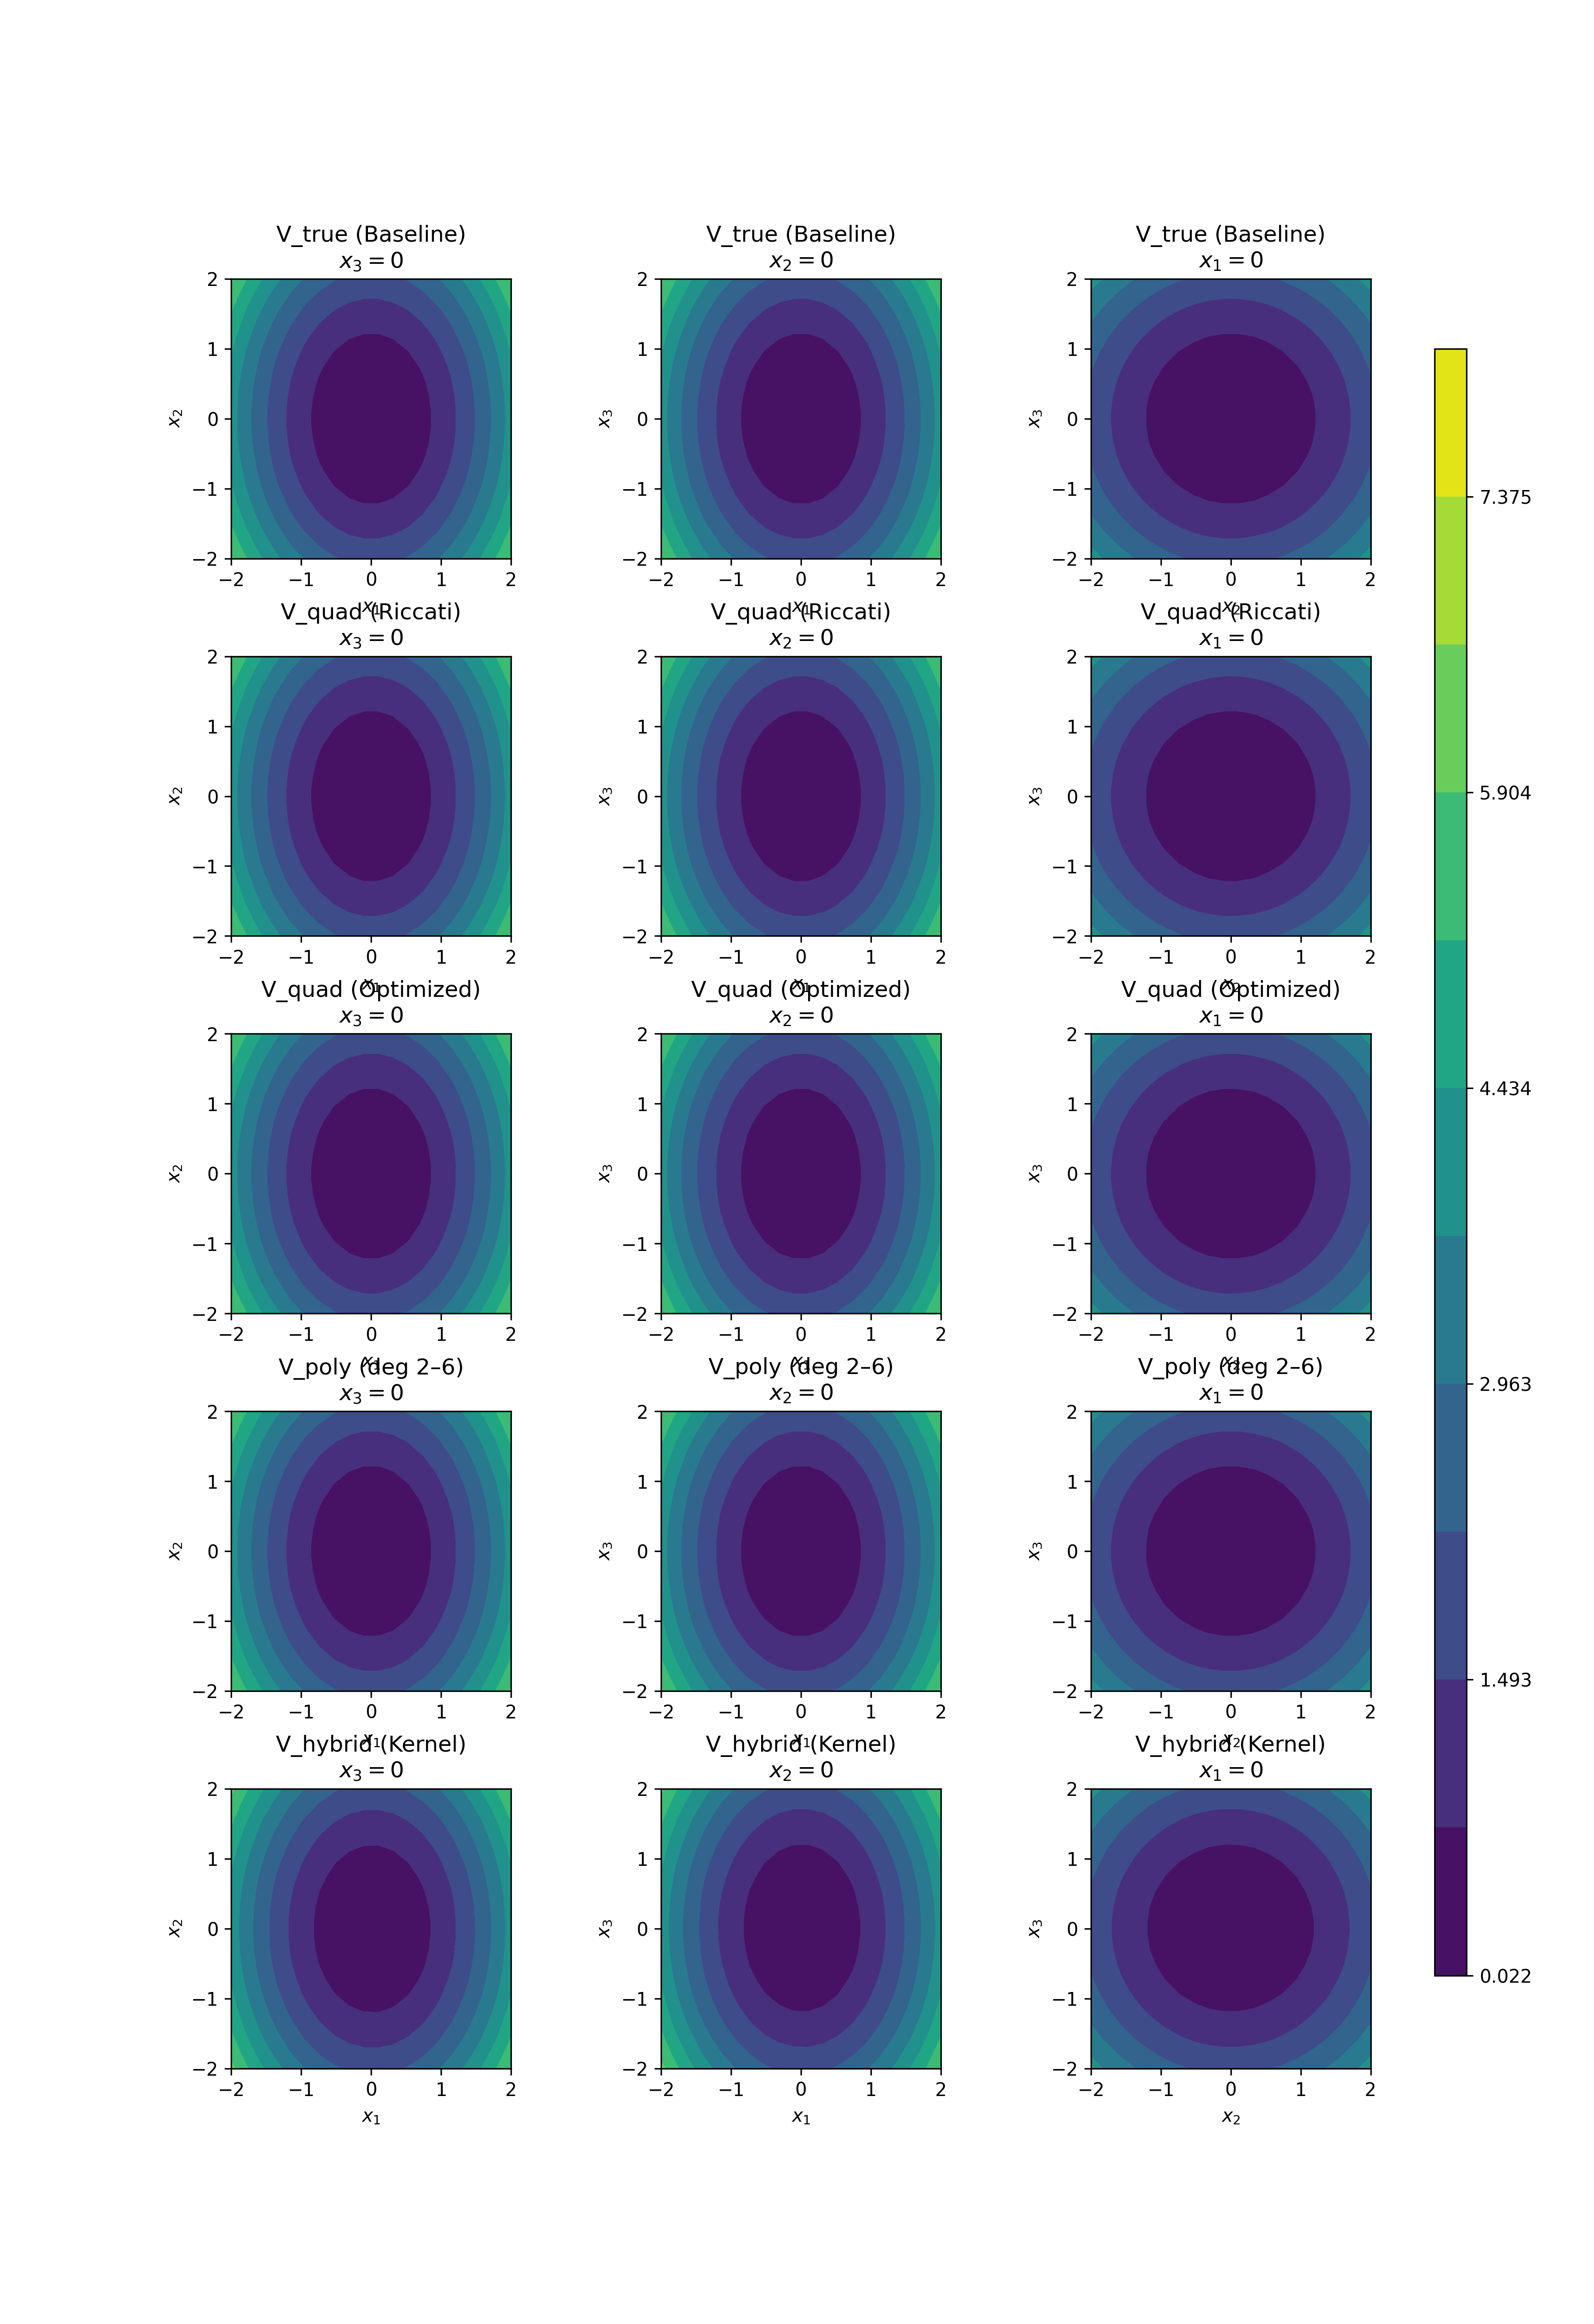
\includegraphics[width=\textwidth]{quasi_potential_slices_sparse.png}
  \caption{Contour slices of the true quasi-potential (Left), the Riccati
  quadratic approximation (Middle), and the Hybrid Kernel approximation (Right)
  for Example~3. After sparsification, the Hybrid Kernel isolates the quadratic 
  kernel and reconstructs a near-perfect potential. \textcolor{red}{The corresponding spatial 
  residuals $|V_h - V_{\mathrm{true}}|$ are shown in Figure~\ref{fig:residuals_example3}.}}
  \label{fig:comparison_example3}
\end{figure}

% Figure showing spatial residuals for Example 3
\begin{figure}[htbp]
  \centering
  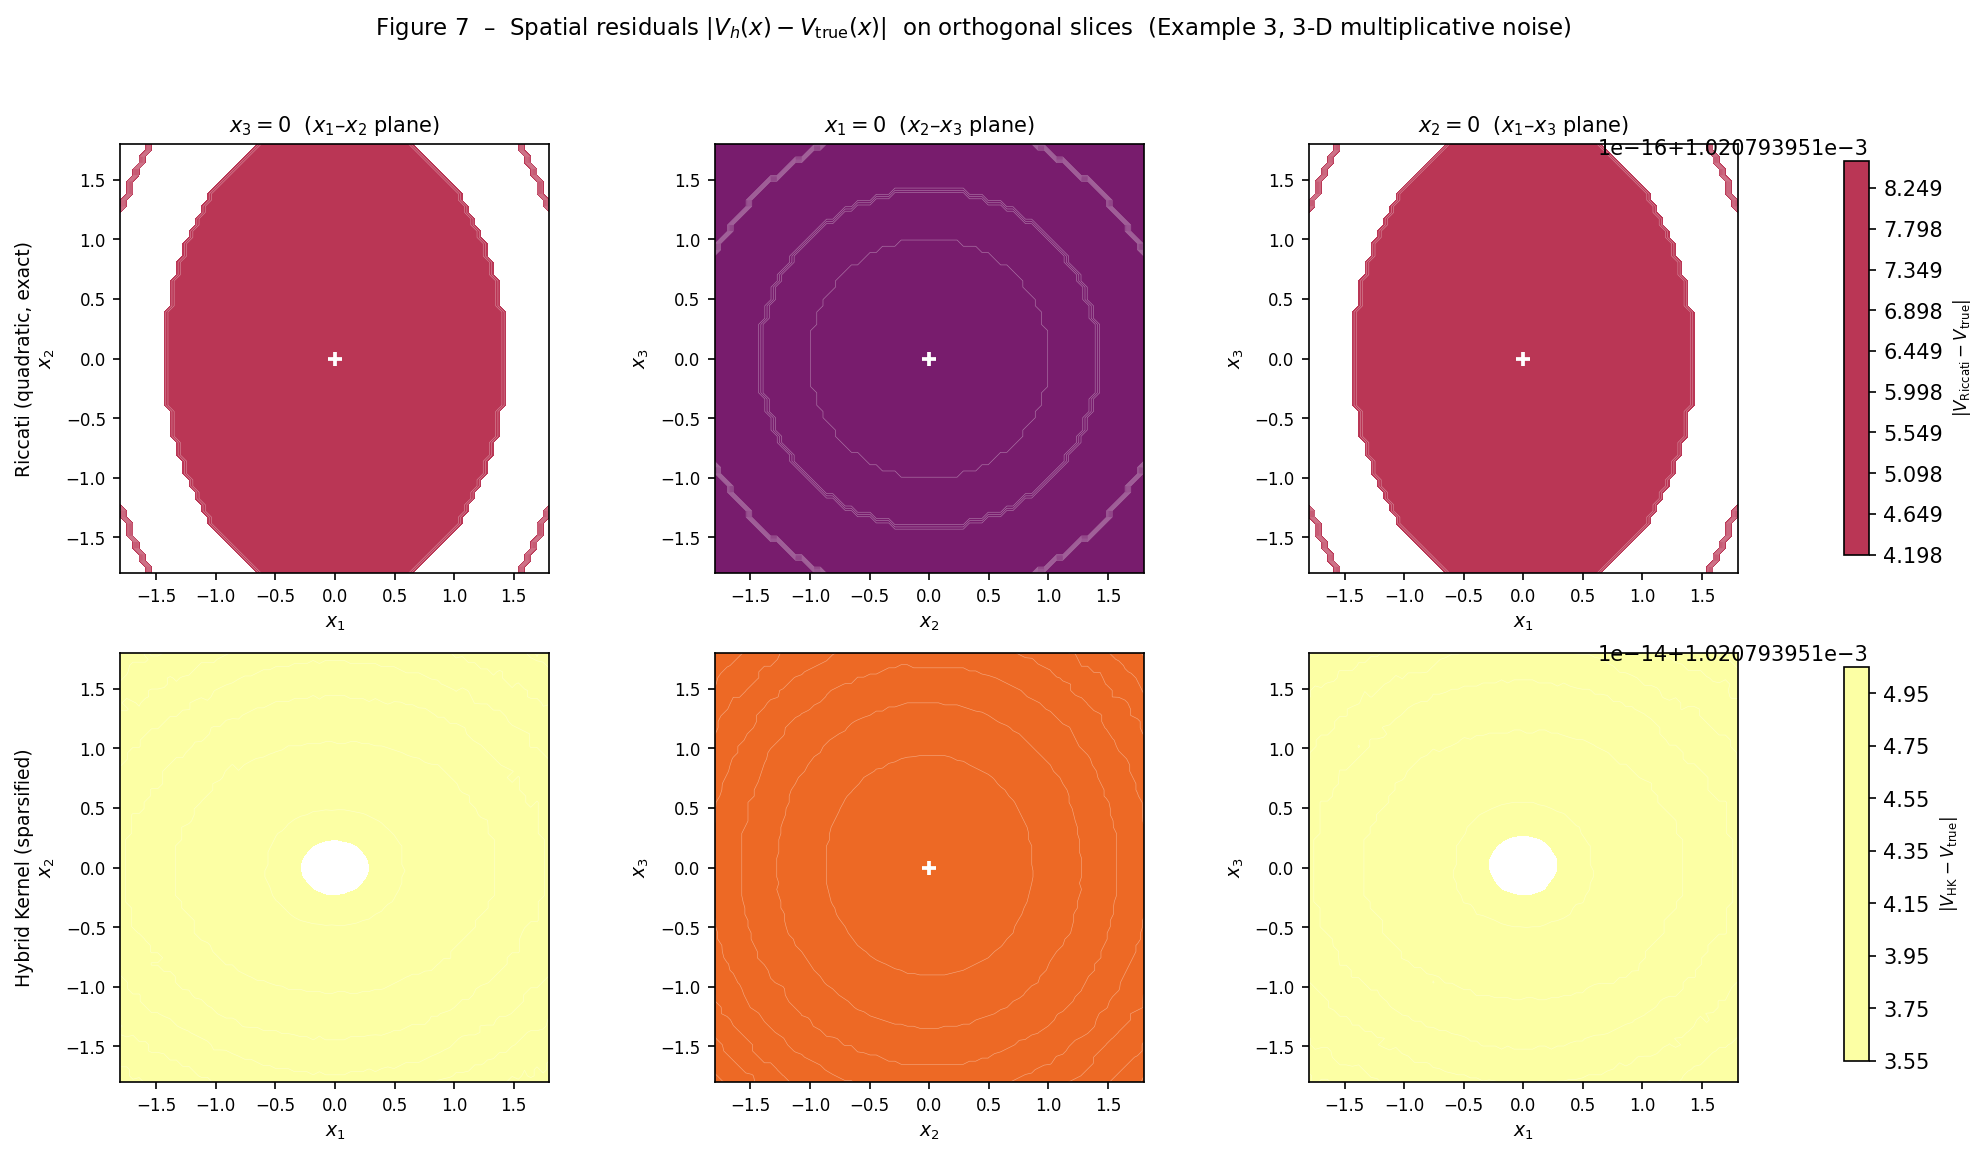
\includegraphics[width=\textwidth]{residuals_example3.png}
  \caption{\textcolor{red}{Spatial residuals $|V_h - V_{\mathrm{true}}|$ for Example~3 on three orthogonal slices ($x_3=0$, $x_1=0$, $x_2=0$). Top row: Riccati (quadratic) approximation residuals, which achieve RMSE $\approx 10^{-3}$ since the true quasi-potential is exactly quadratic and the Riccati matrix captures this structure precisely. Bottom row: Hybrid Kernel approximation residuals, matching the Riccati accuracy (RMSE $\approx 10^{-3}$) after sparsification. Starting from a dictionary of 19 features (monomials up to degree~3), the $\ell_1$ penalty automatically zeroes out all but three terms---precisely $x_1^2$, $x_2^2$, and $x_3^2$---recovering the true quadratic structure without prior knowledge of its form. Separate colorscales are used for each row; both are on the order of $10^{-3}$, confirming that errors are negligible throughout the domain.}}
  \label{fig:residuals_example3}
\end{figure}

\section{Conclusion}

\textcolor{red}{We have presented a kernel-based framework for computing quasi-potentials in stochastic dynamical systems. The method parameterizes Koopman eigenfunctions via RKHS ansätze and minimizes a composite loss~\eqref{eq:composite_loss} that simultaneously enforces the Hamilton--Jacobi equation, matches the local Hessian to the Riccati solution, and promotes kernel sparsity through $\ell_1$ regularization. The result is an analytical surrogate that is cheap to evaluate and automatically selects the correct functional form through sparsification.}

\textcolor{red}{Theorem~\ref{thm:consistency-curvature} establishes consistency of the learned surrogate with the true quasi-potential as the collocation count $N$ grows, with convergence guaranteed in function values, gradients, and equilibrium curvature. Three benchmark examples validate the approach: Example~1 (two-dimensional gradient system) demonstrates kernel sparsification; Example~2 (double-well with non-trivial topology) shows that the hybrid surrogate improves upon the Riccati baseline; and Example~3 (three-dimensional multiplicative noise) confirms automatic recovery of the exact quadratic structure (RMSE $\approx 10^{-3}$, matching the Riccati baseline) and an empirical convergence rate $\text{RMSE}\sim N^{-0.73}$ consistent with kernel collocation theory.}

\paragraph{Limitations and future work.}
\textcolor{red}{The main limitation of the current work is the absence of a head-to-head comparison with established methods such as ordered-upwind methods~\cite{cameron2012finding, dahiya2018ordered}, string methods~\cite{heymann2008geometric, grafke2019numerical}, and geometric minimum action approaches~\cite{zhou2008adaptive}. Such a comparison, which would require careful tuning of each method on common test problems, is left as an important direction for future work.
Computational cost scales as $O(N^2 n)$, limiting applicability beyond $n\approx 5$--8 dimensions with current implementations; sparse collocation, reduced-order modeling, and hierarchical kernel architectures are promising mitigation strategies. Extensions to non-Gaussian or Lévy noise, globally consistent multi-basin reconstruction, and the fully data-driven setting (where drift and diffusion must themselves be estimated) also remain open.}

\section*{Acknowledgments}	
The authors acknowledge support from the National Natural Science Foundation of China (Grant Nos. 12302035, 12572038, and 12372030) and Fundamental Research Funds for the Central Universities (Grant No. 30925010411).

\bibliographystyle{abbrv}
\bibliography{references,references_quasi_potential}

\end{document}

